% -----------------------------------------------------------------------------
\section{SBOL Visual Glyphs}\label{apdx:symbols}
% -----------------------------------------------------------------------------

The following pages present all current glyphs for SBOL Visual, organized by glyph families.
Each entry lists:
\begin{itemize}
\item Glyph family name
\item Associated ontology terms
\item Recommended and alternate glyphs
\item At least one example of when this glyph would be used
\item Any additional notes
\end{itemize}

\subsection{Sequence Feature Glyphs}\label{apdx:sym:feature}

These glyphs represent features of nucleic acid sequences, and include a bounding box (grey dashed box) and a recommended alignment to the nucleic acid backbone (grey dashed horizontal line).

% Autogenerated glyph page collection, do not edit by hand

\includepdf[pagecommand={}]{glyphscript/Glyphs/aptamer.pdf}

\includepdf[pagecommand={}]{glyphscript/Glyphs/assembly-scar.pdf}

\includepdf[pagecommand={}]{glyphscript/Glyphs/blunt-restriction-site.pdf}
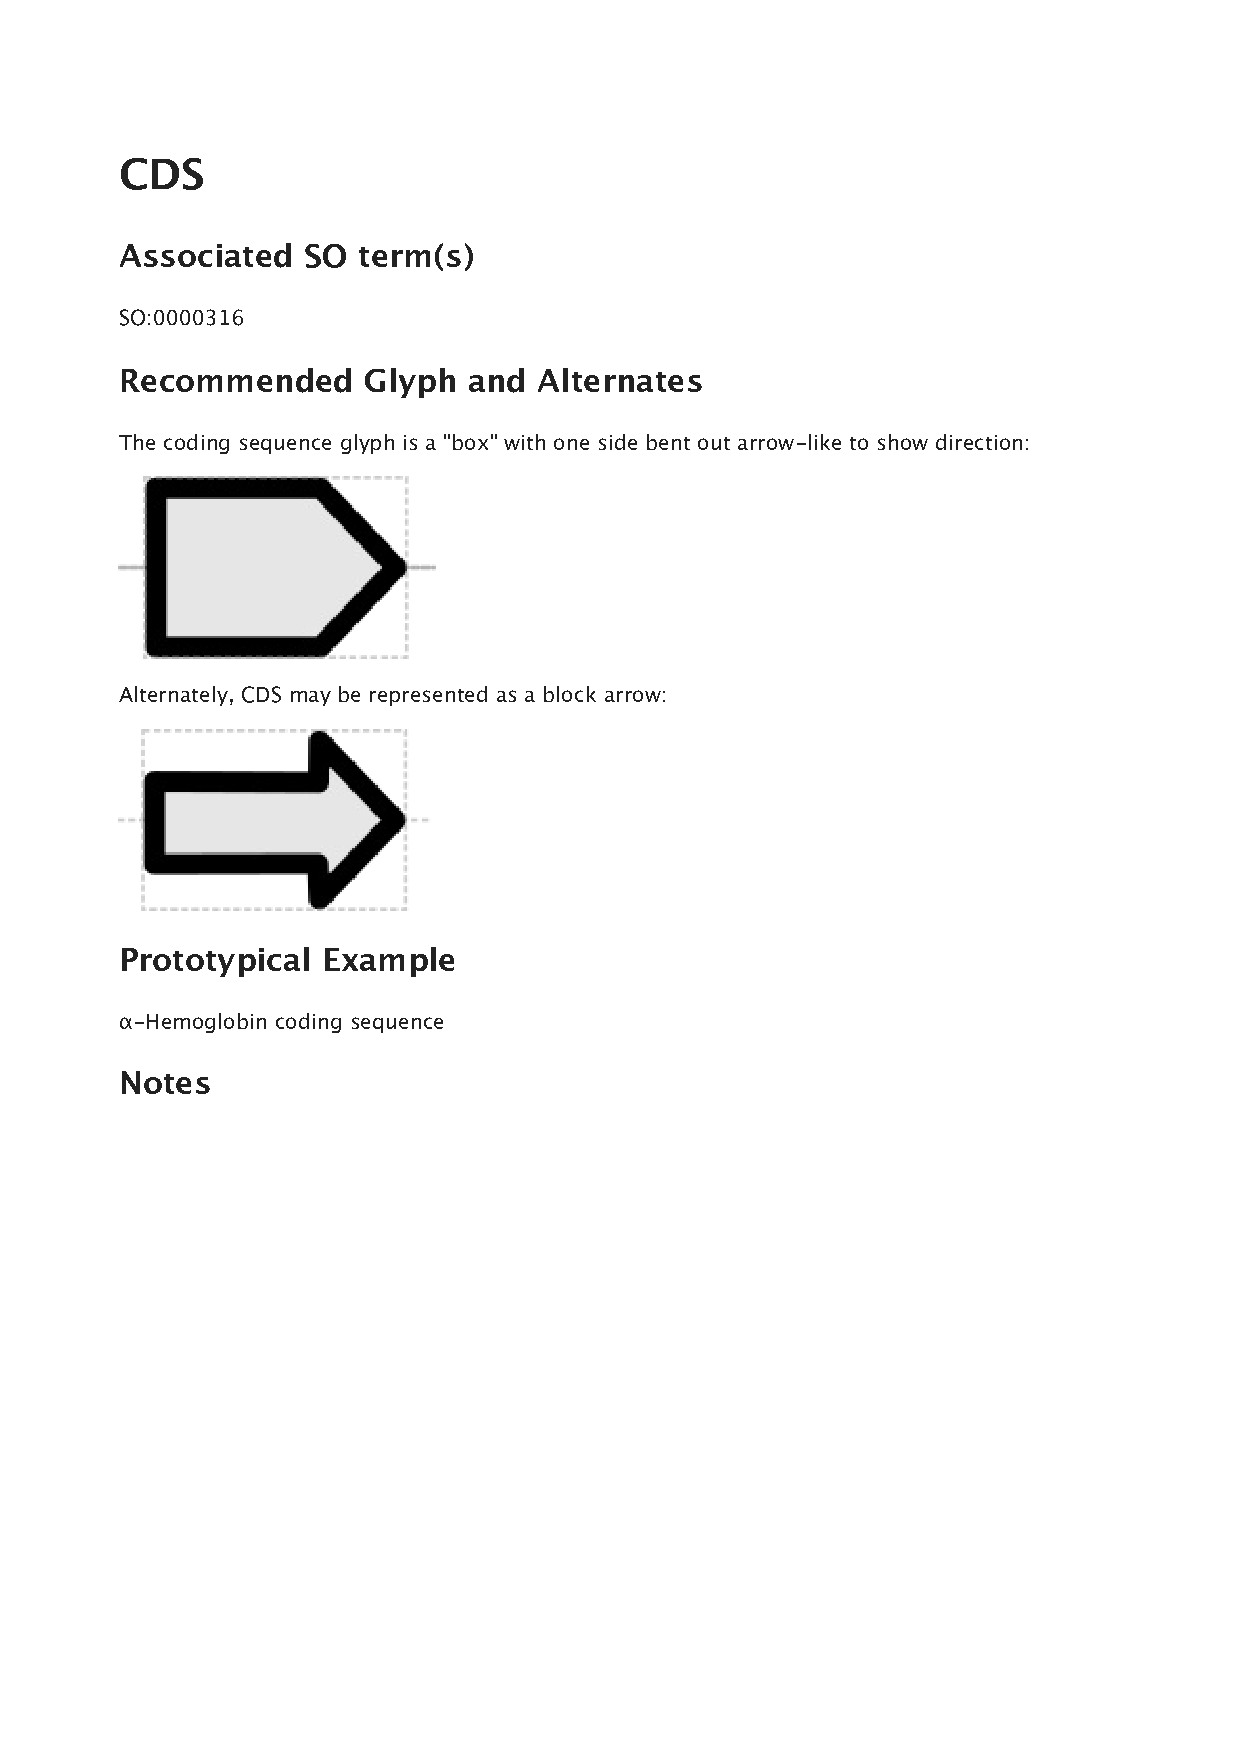
\includepdf[pagecommand={}]{glyphscript/Glyphs/cds.pdf}
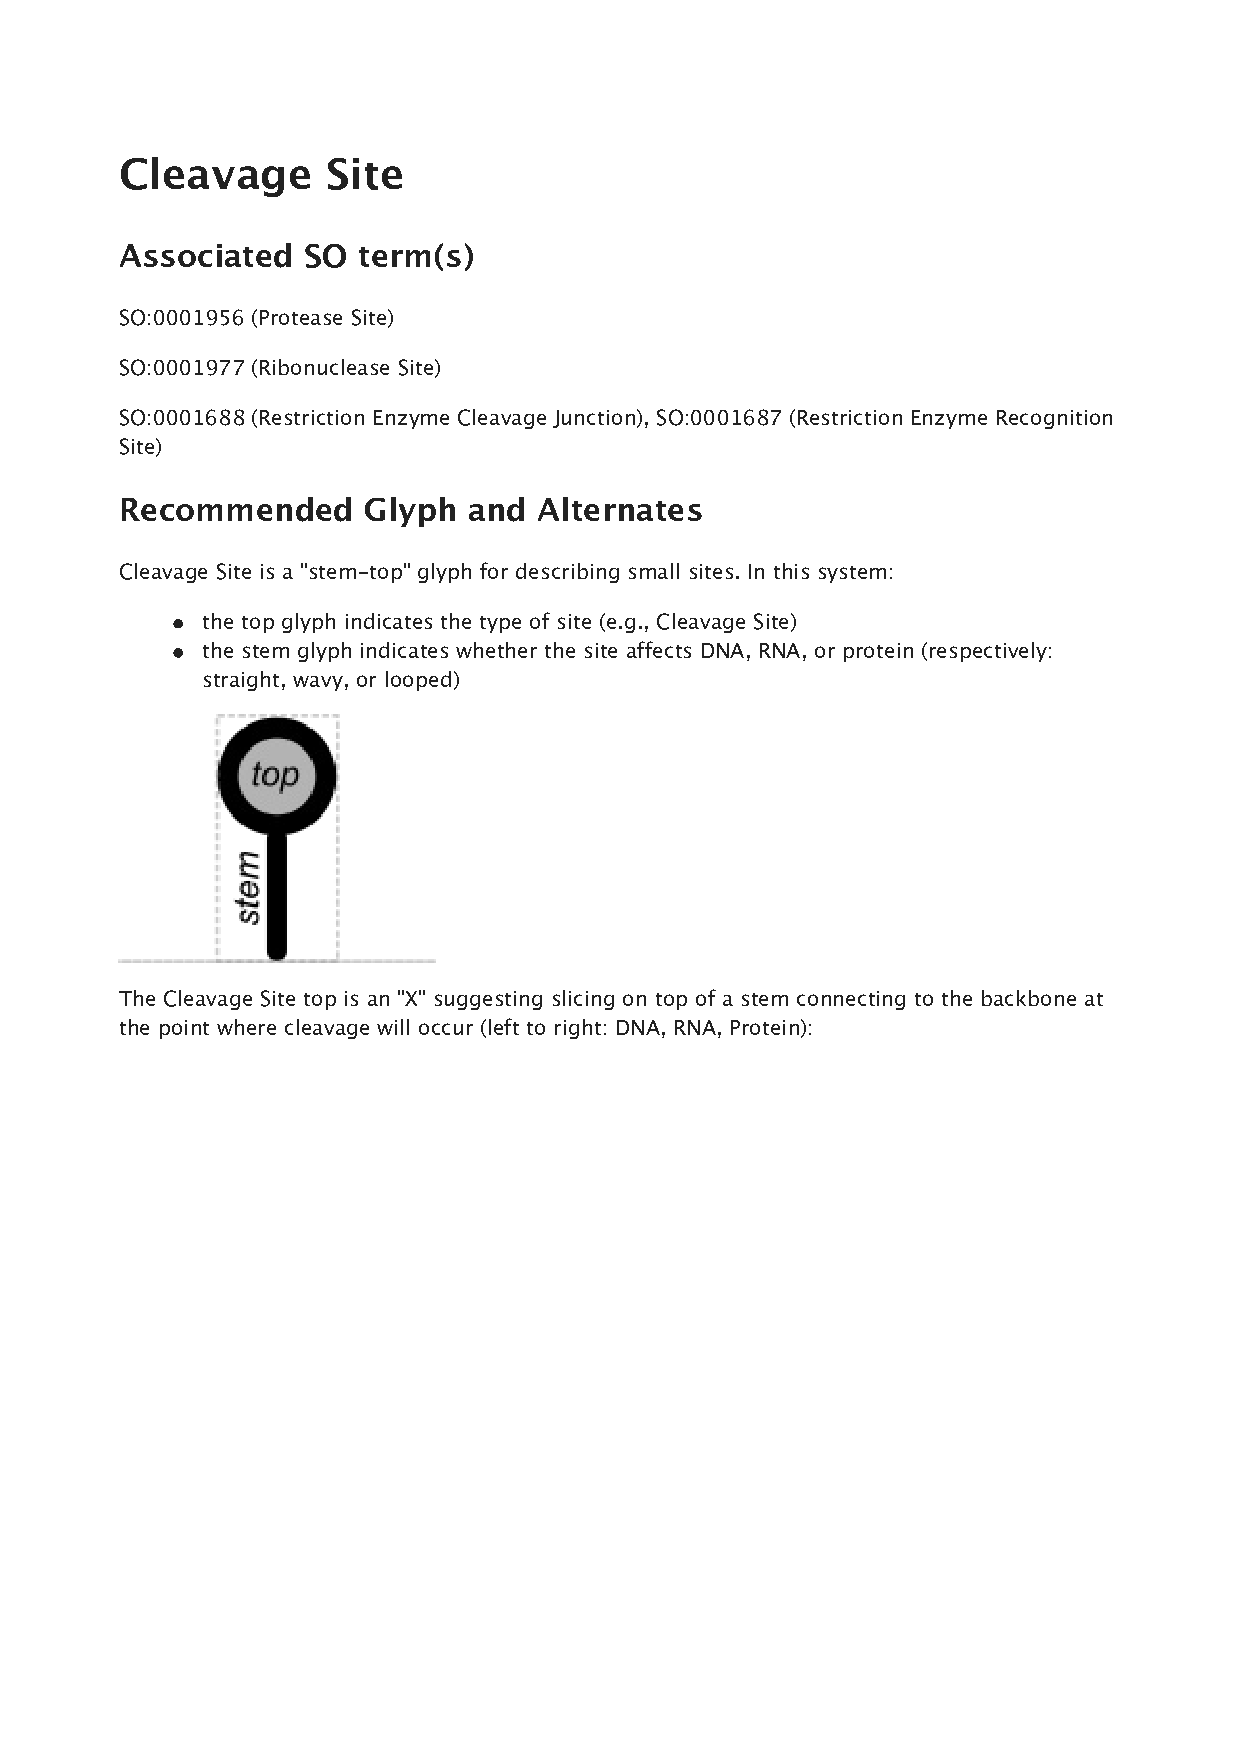
\includepdf[pagecommand={}]{glyphscript/Glyphs/cleavage-site.pdf}
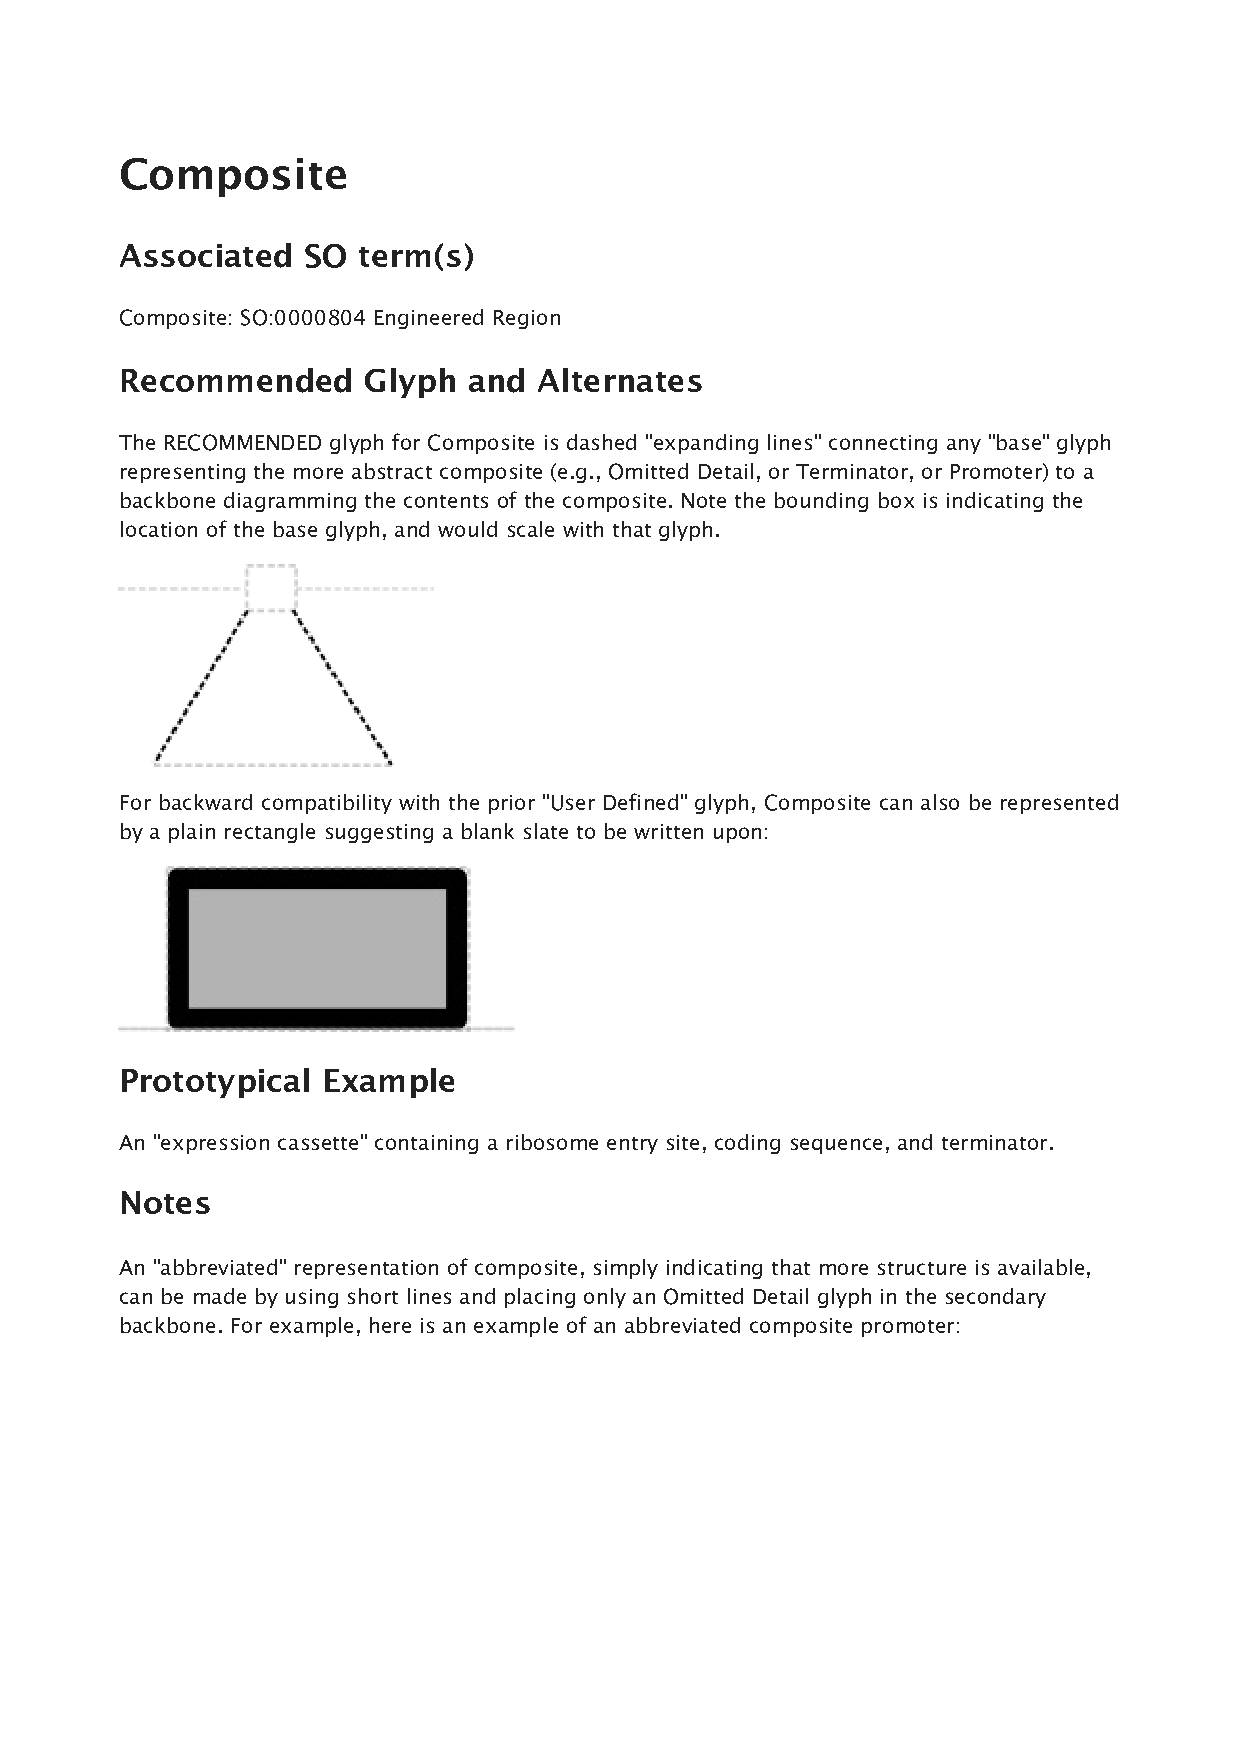
\includepdf[pagecommand={}]{glyphscript/Glyphs/composite.pdf}

\includepdf[pagecommand={}]{glyphscript/Glyphs/five-prime-overhang.pdf}

\includepdf[pagecommand={}]{glyphscript/Glyphs/five-prime-sticky-restriction-site.pdf}

\includepdf[pagecommand={}]{glyphscript/Glyphs/insulator.pdf}
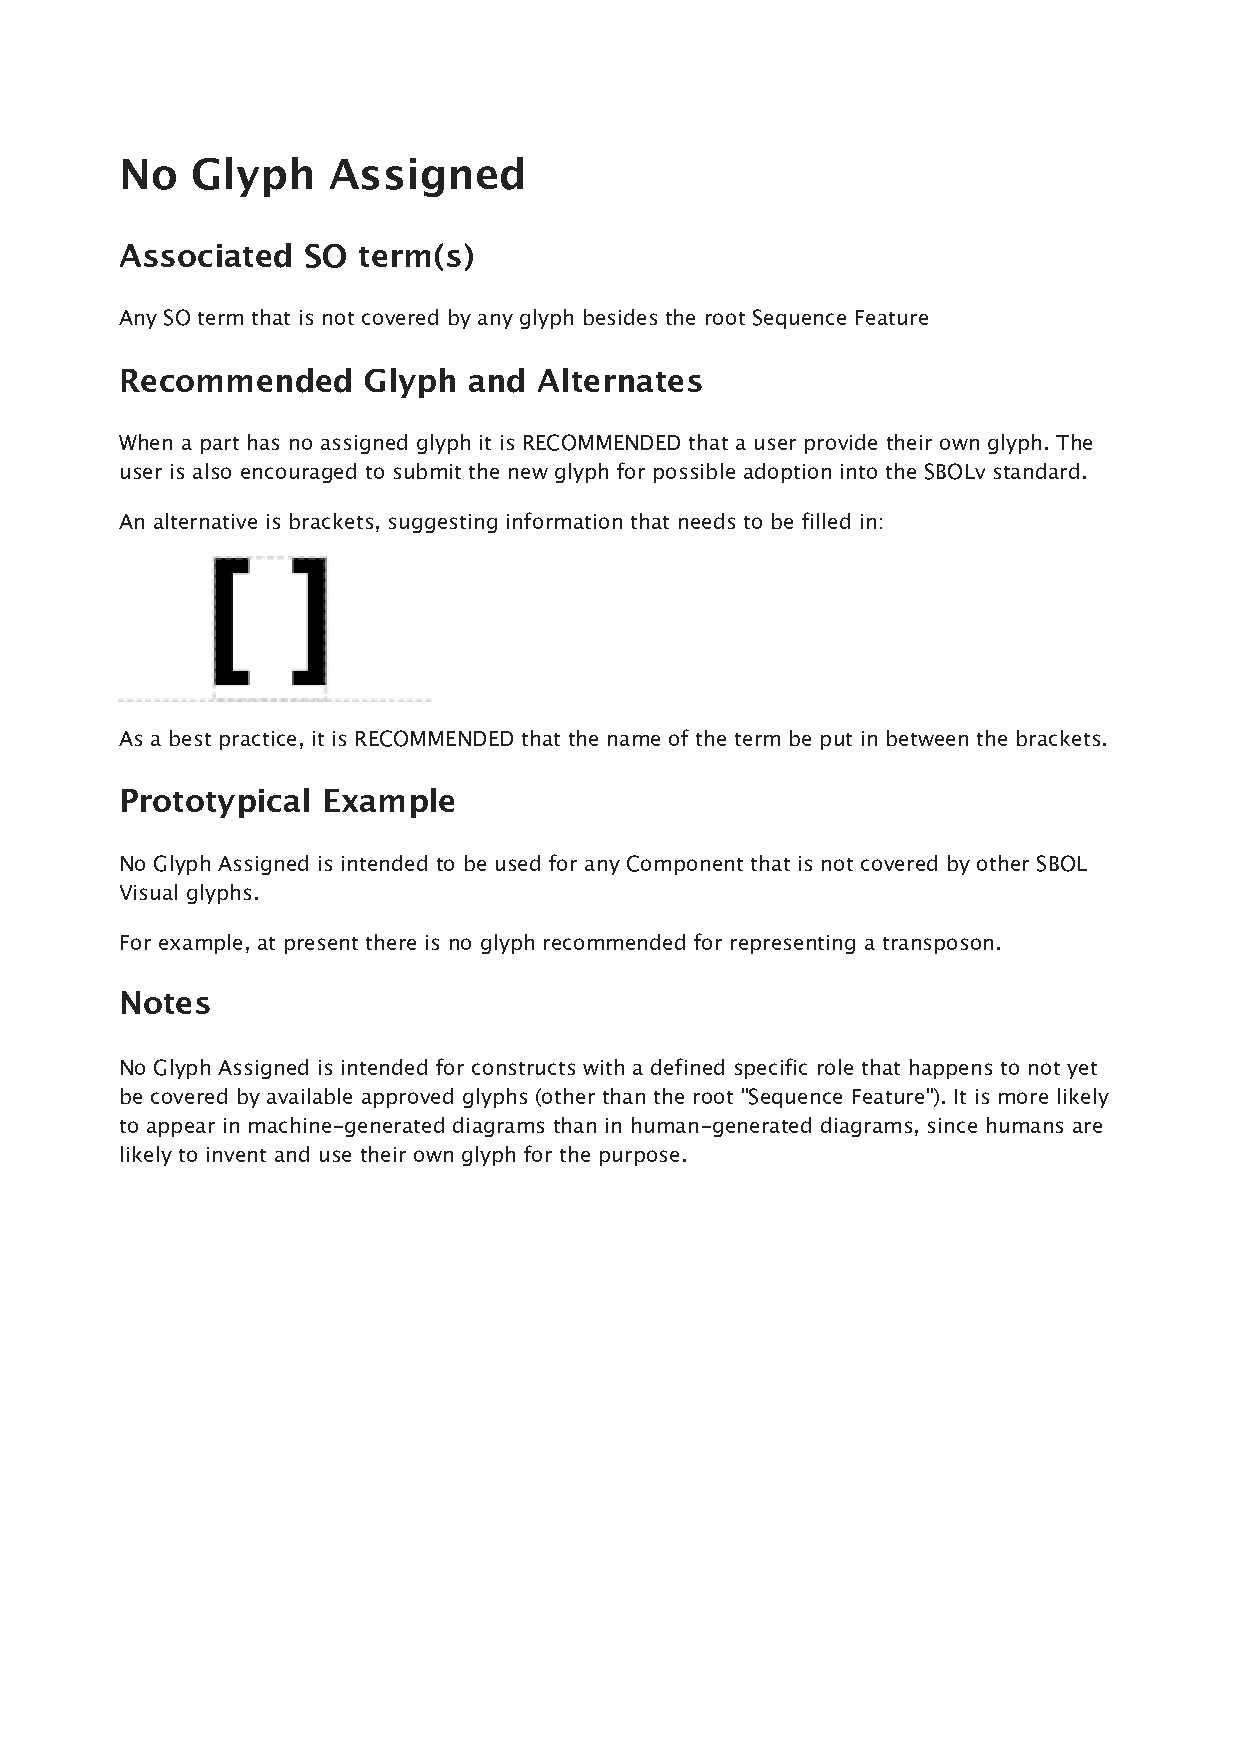
\includepdf[pagecommand={}]{glyphscript/Glyphs/no-glyph-assigned.pdf}

\includepdf[pagecommand={}]{glyphscript/Glyphs/omitted-detail.pdf}
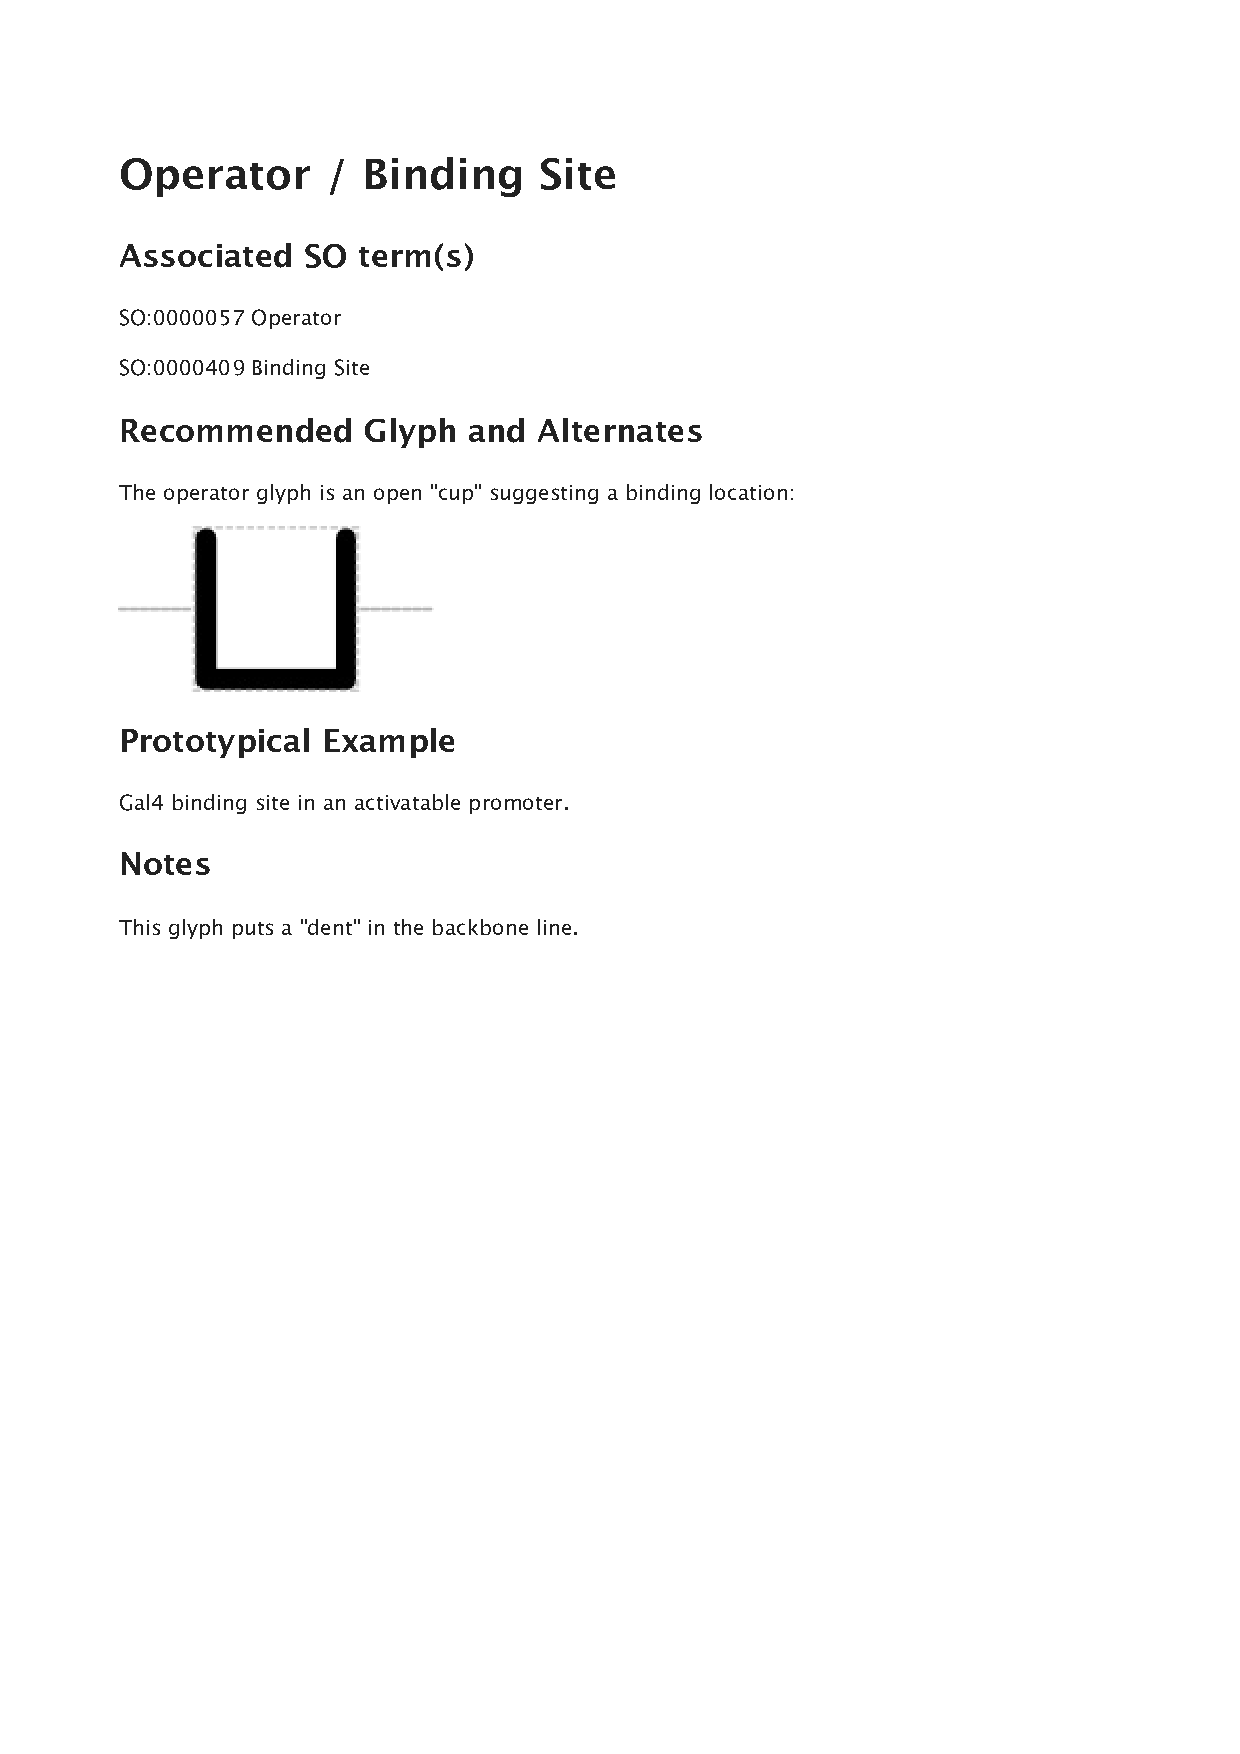
\includepdf[pagecommand={}]{glyphscript/Glyphs/operator.pdf}
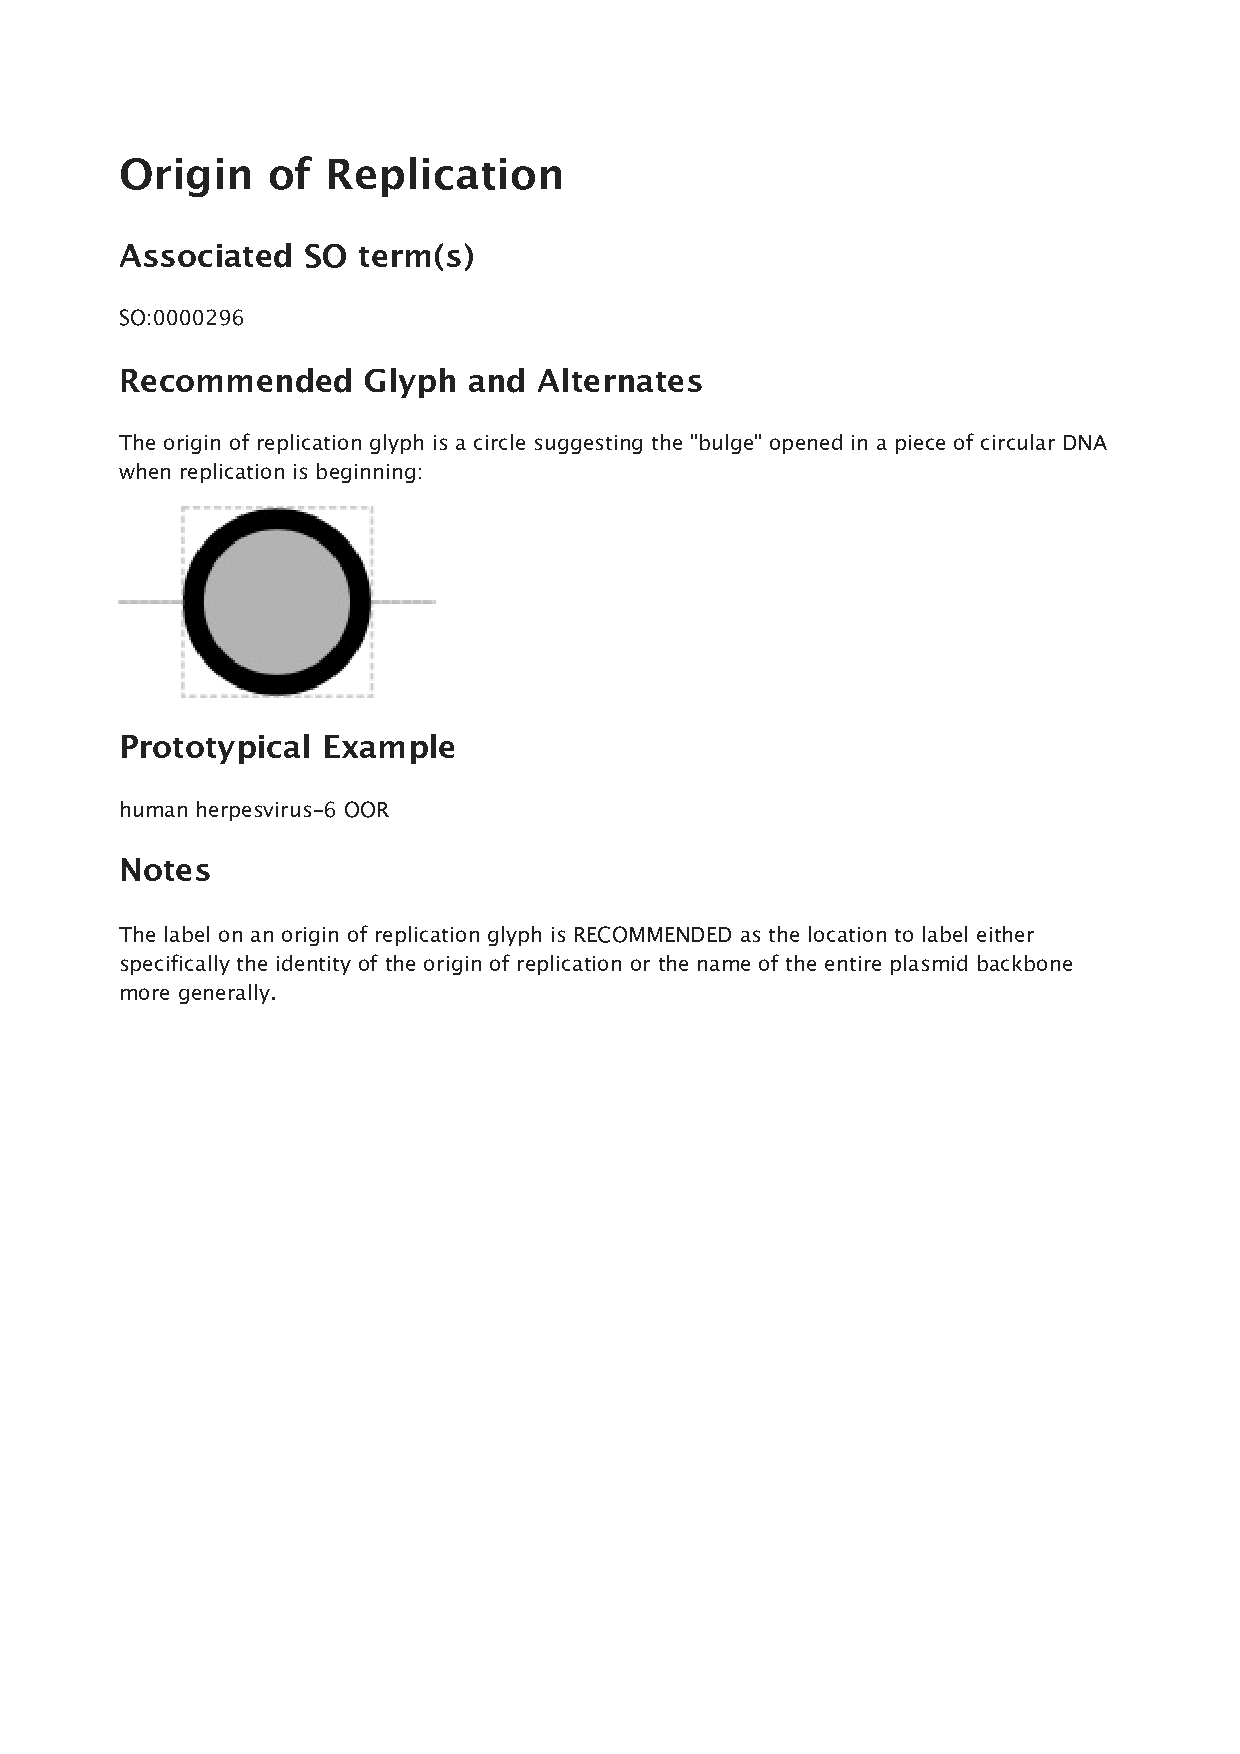
\includepdf[pagecommand={}]{glyphscript/Glyphs/origin-of-replication.pdf}

\includepdf[pagecommand={}]{glyphscript/Glyphs/origin-of-transfer.pdf}

\includepdf[pagecommand={}]{glyphscript/Glyphs/polyA.pdf}
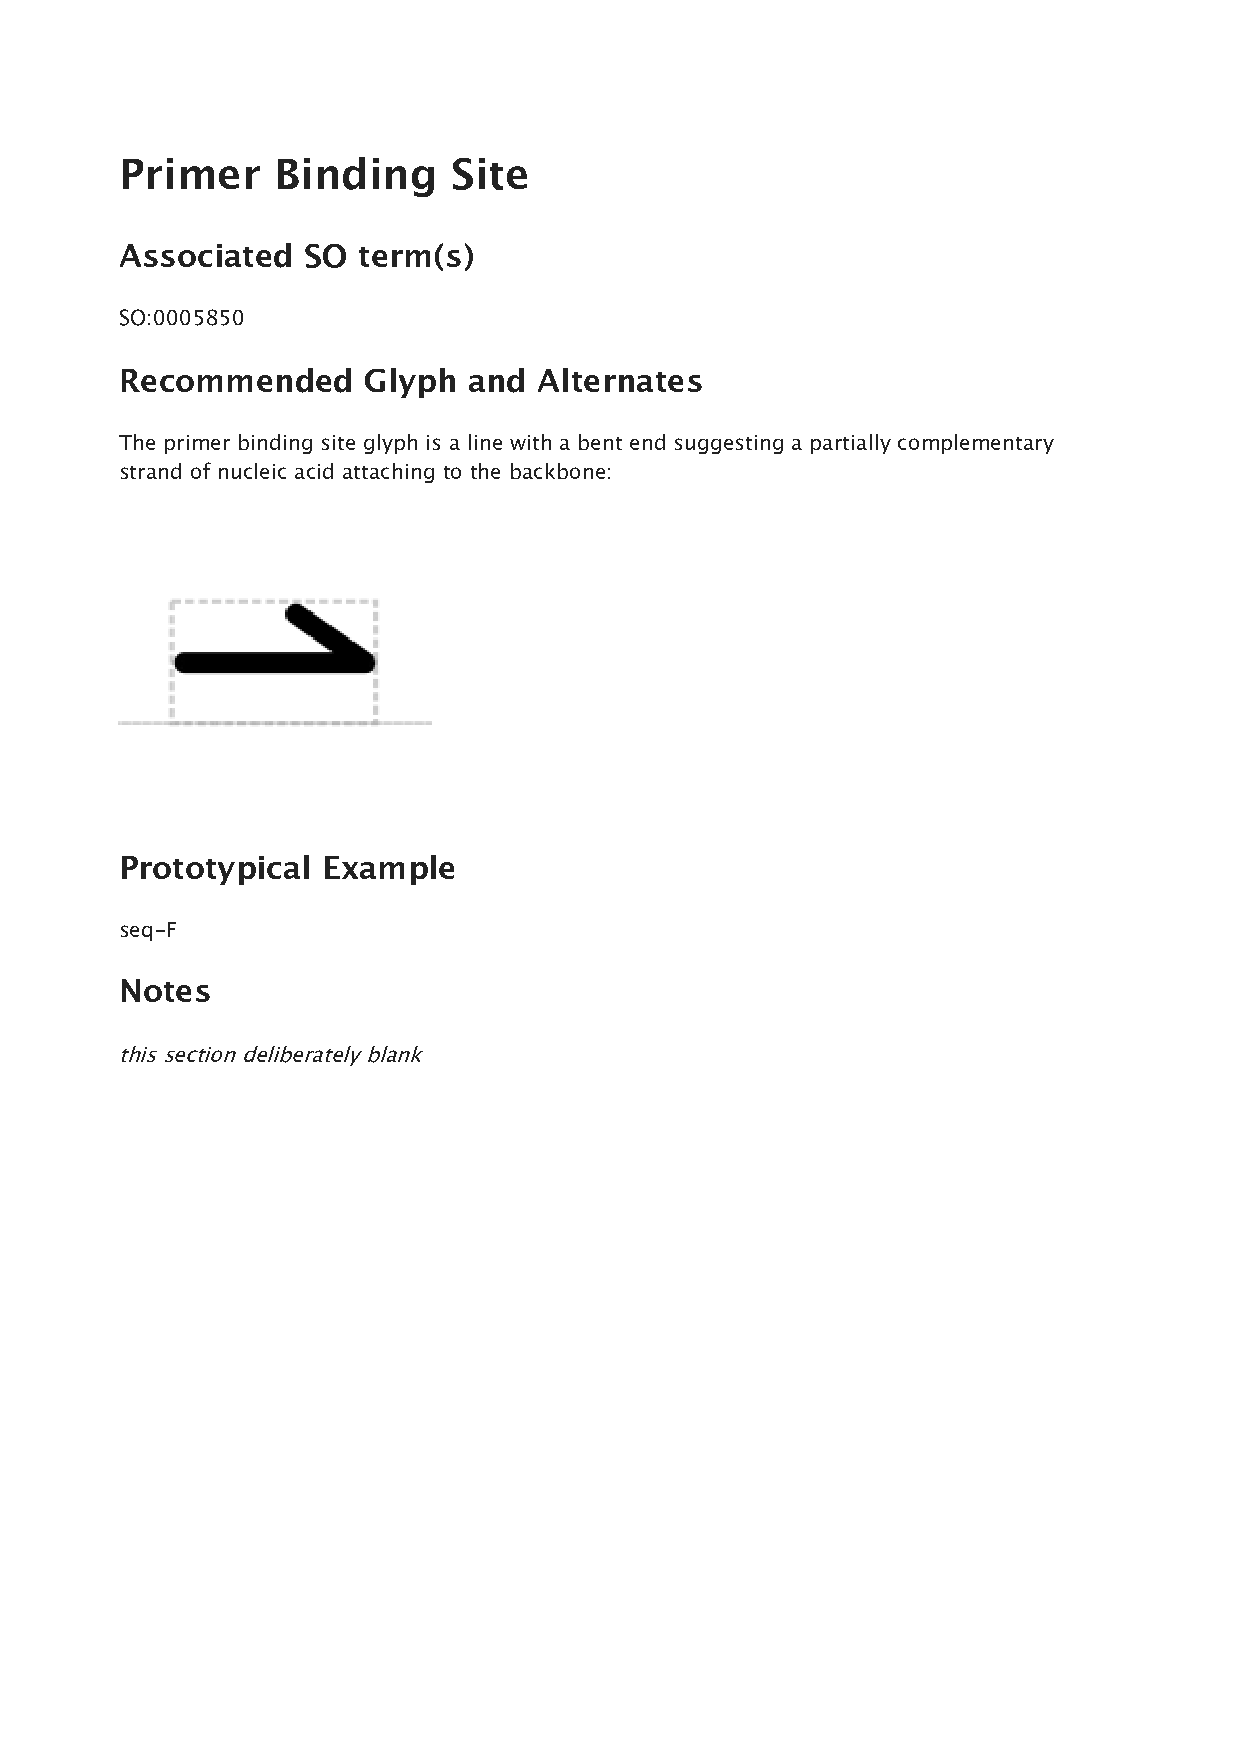
\includepdf[pagecommand={}]{glyphscript/Glyphs/primer-binding-site.pdf}

\includepdf[pagecommand={}]{glyphscript/Glyphs/promoter.pdf}
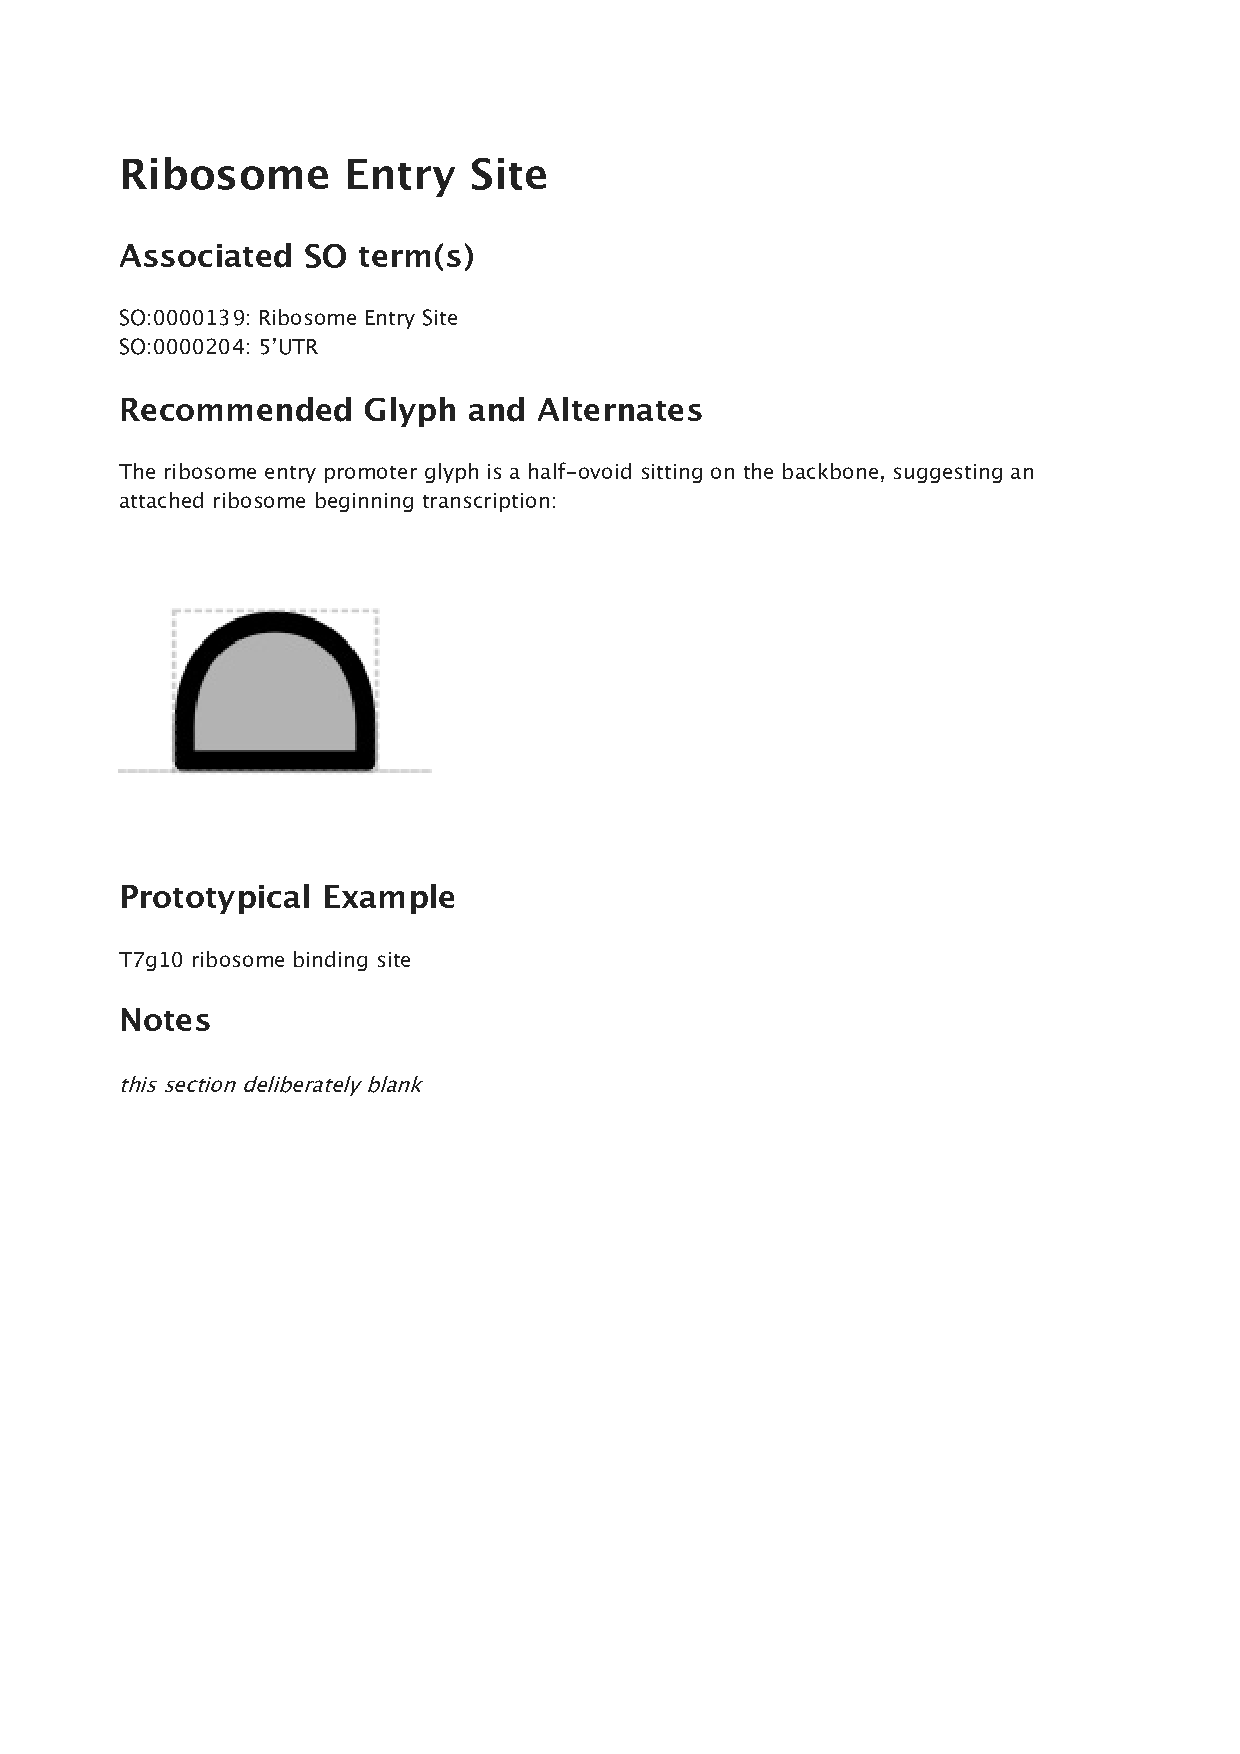
\includepdf[pagecommand={}]{glyphscript/Glyphs/ribosome-entry-site.pdf}

\includepdf[pagecommand={}]{glyphscript/Glyphs/signature.pdf}
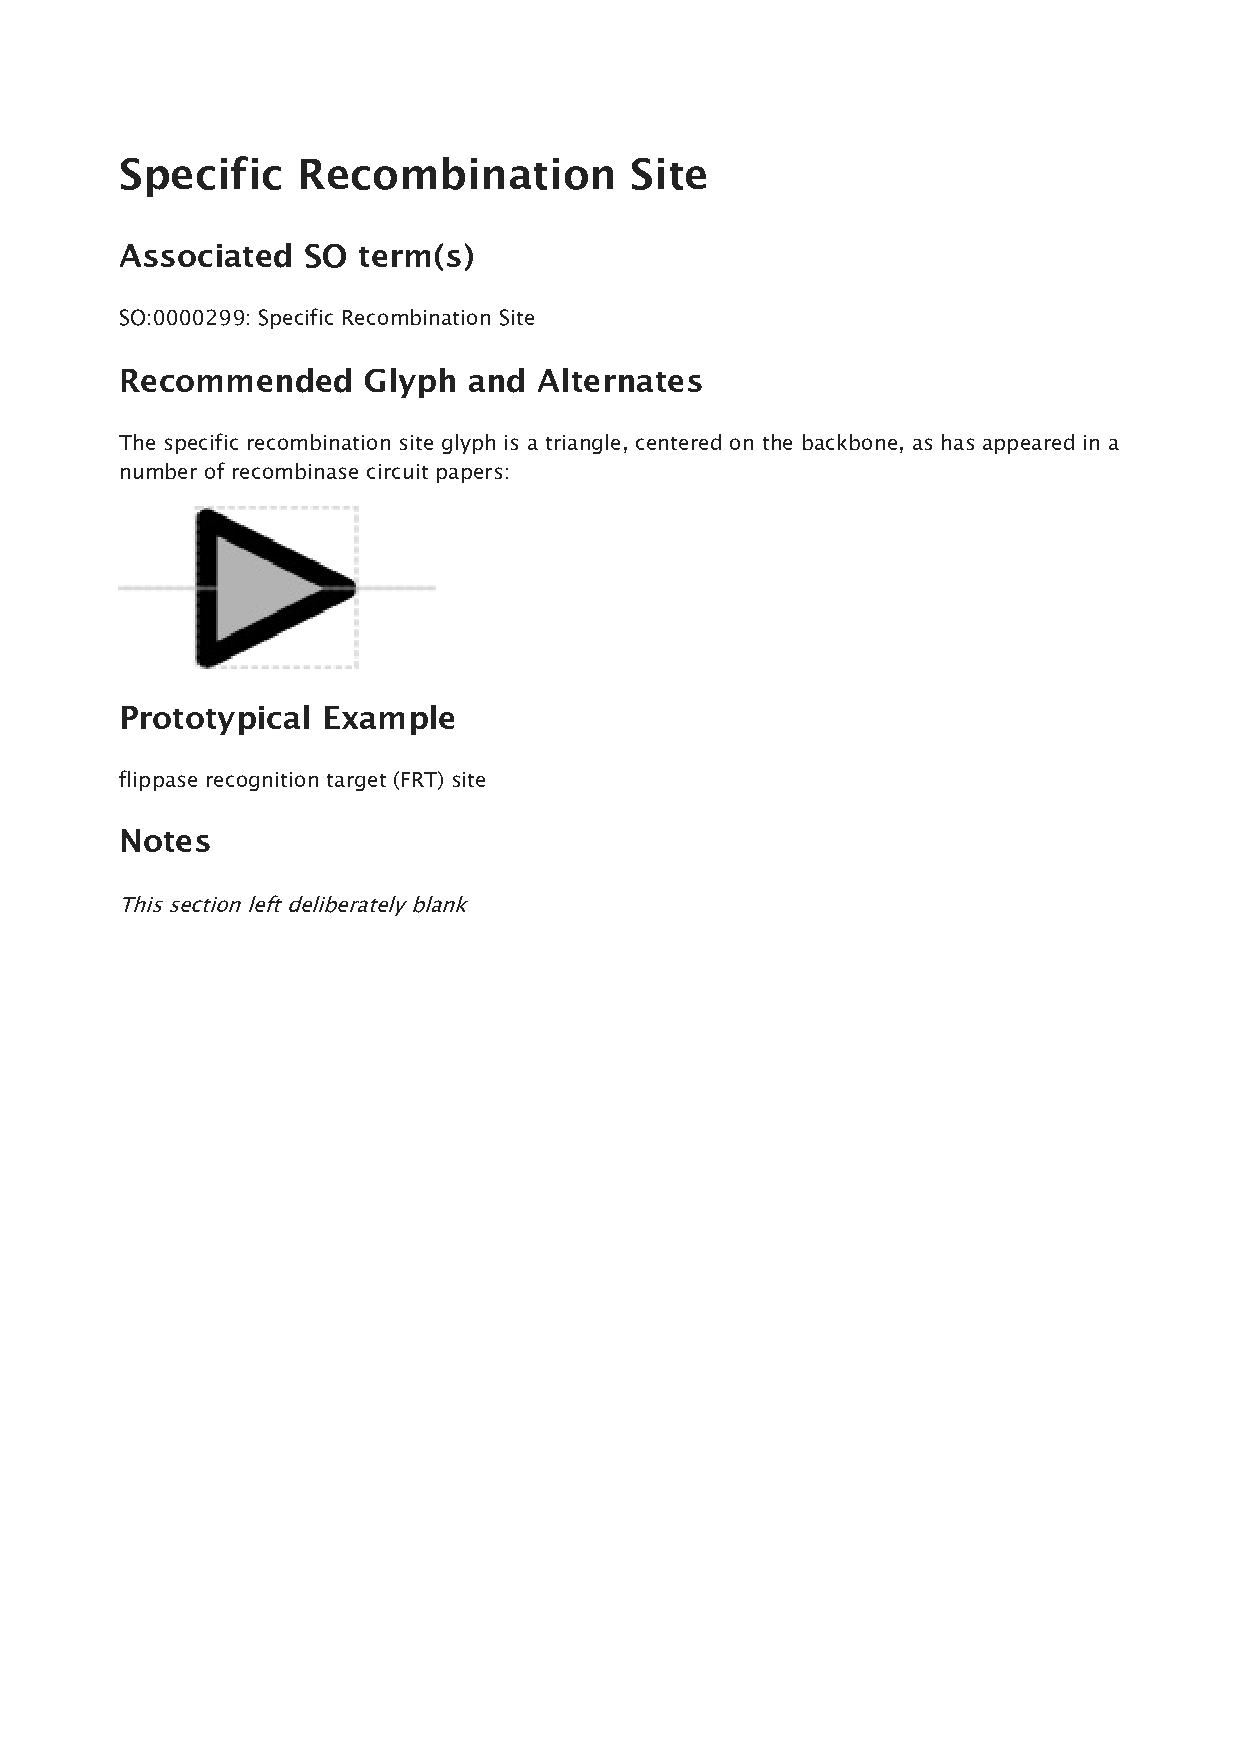
\includepdf[pagecommand={}]{glyphscript/Glyphs/specific-recombination-site.pdf}
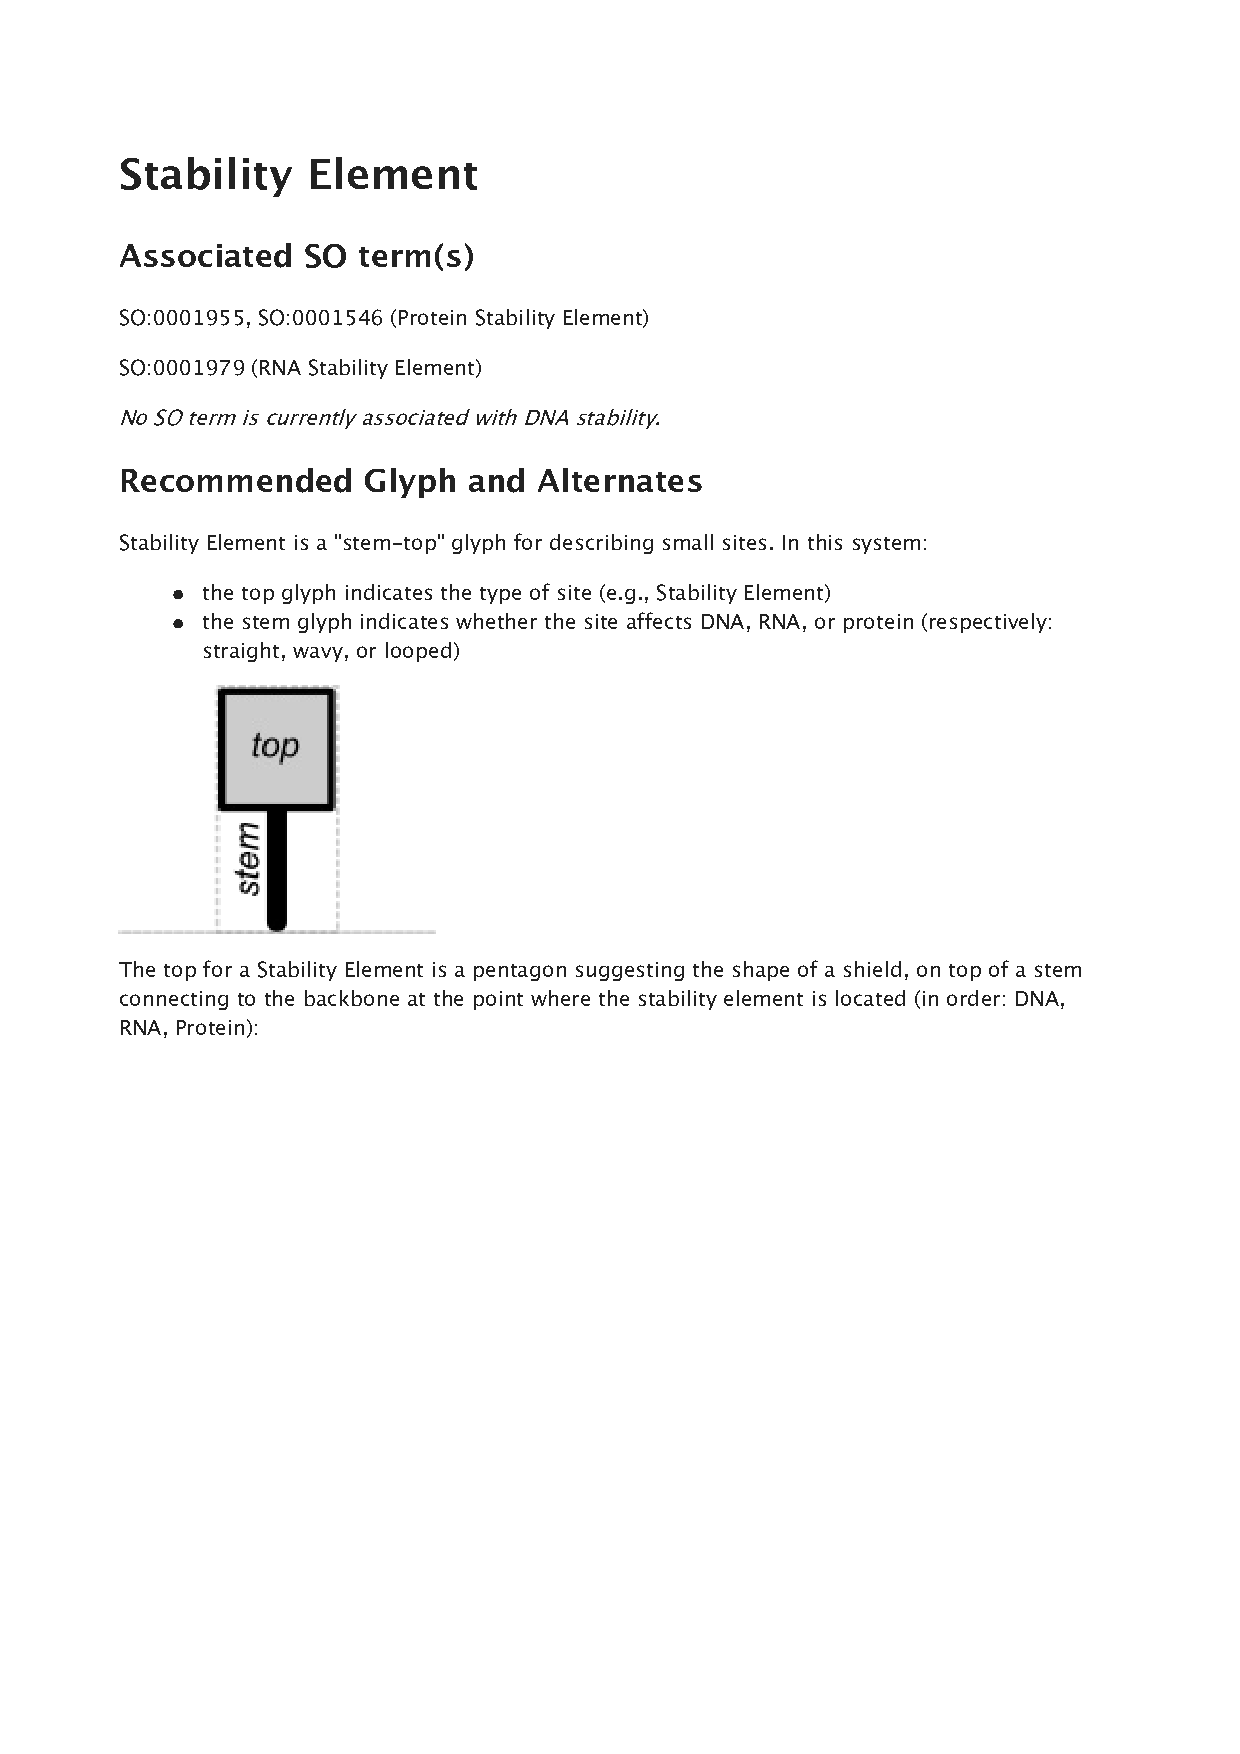
\includepdf[pagecommand={}]{glyphscript/Glyphs/stability-element.pdf}
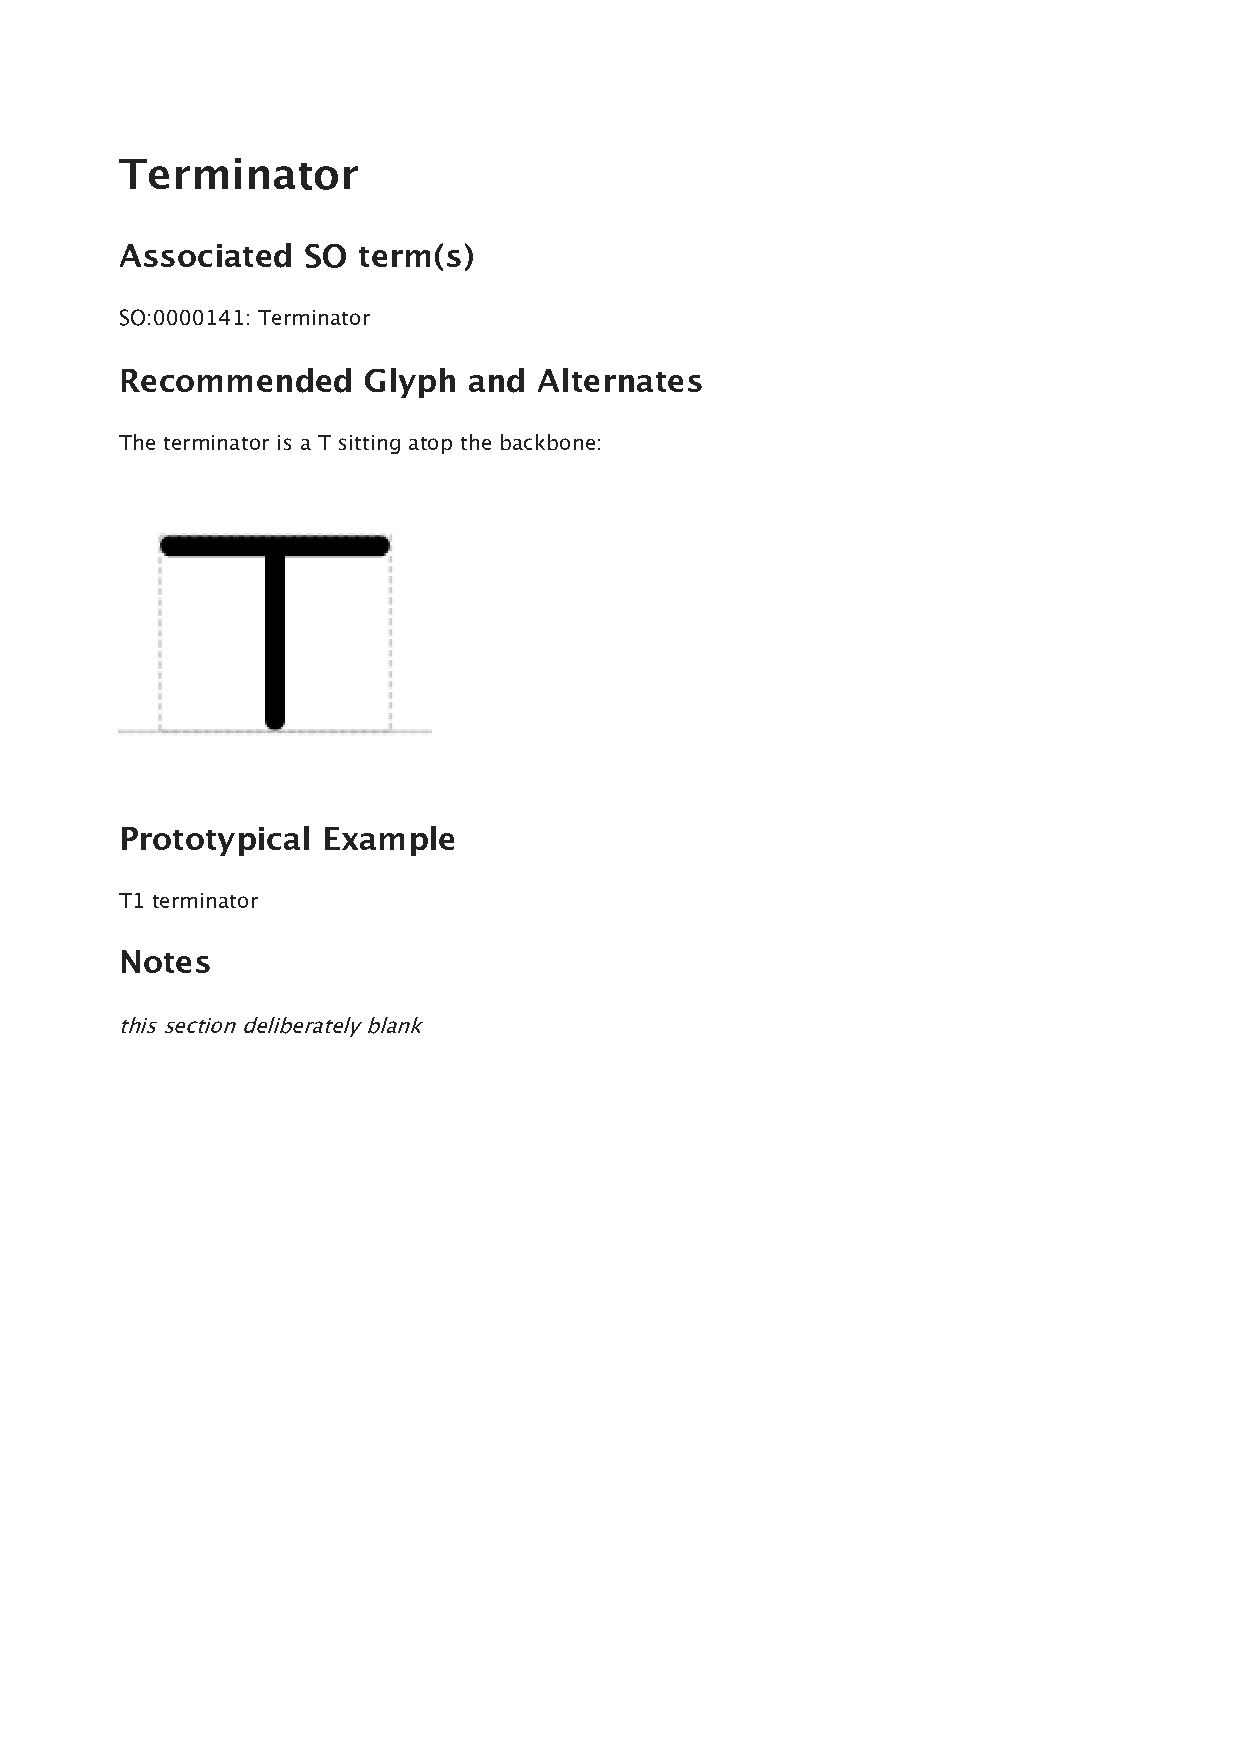
\includepdf[pagecommand={}]{glyphscript/Glyphs/terminator.pdf}
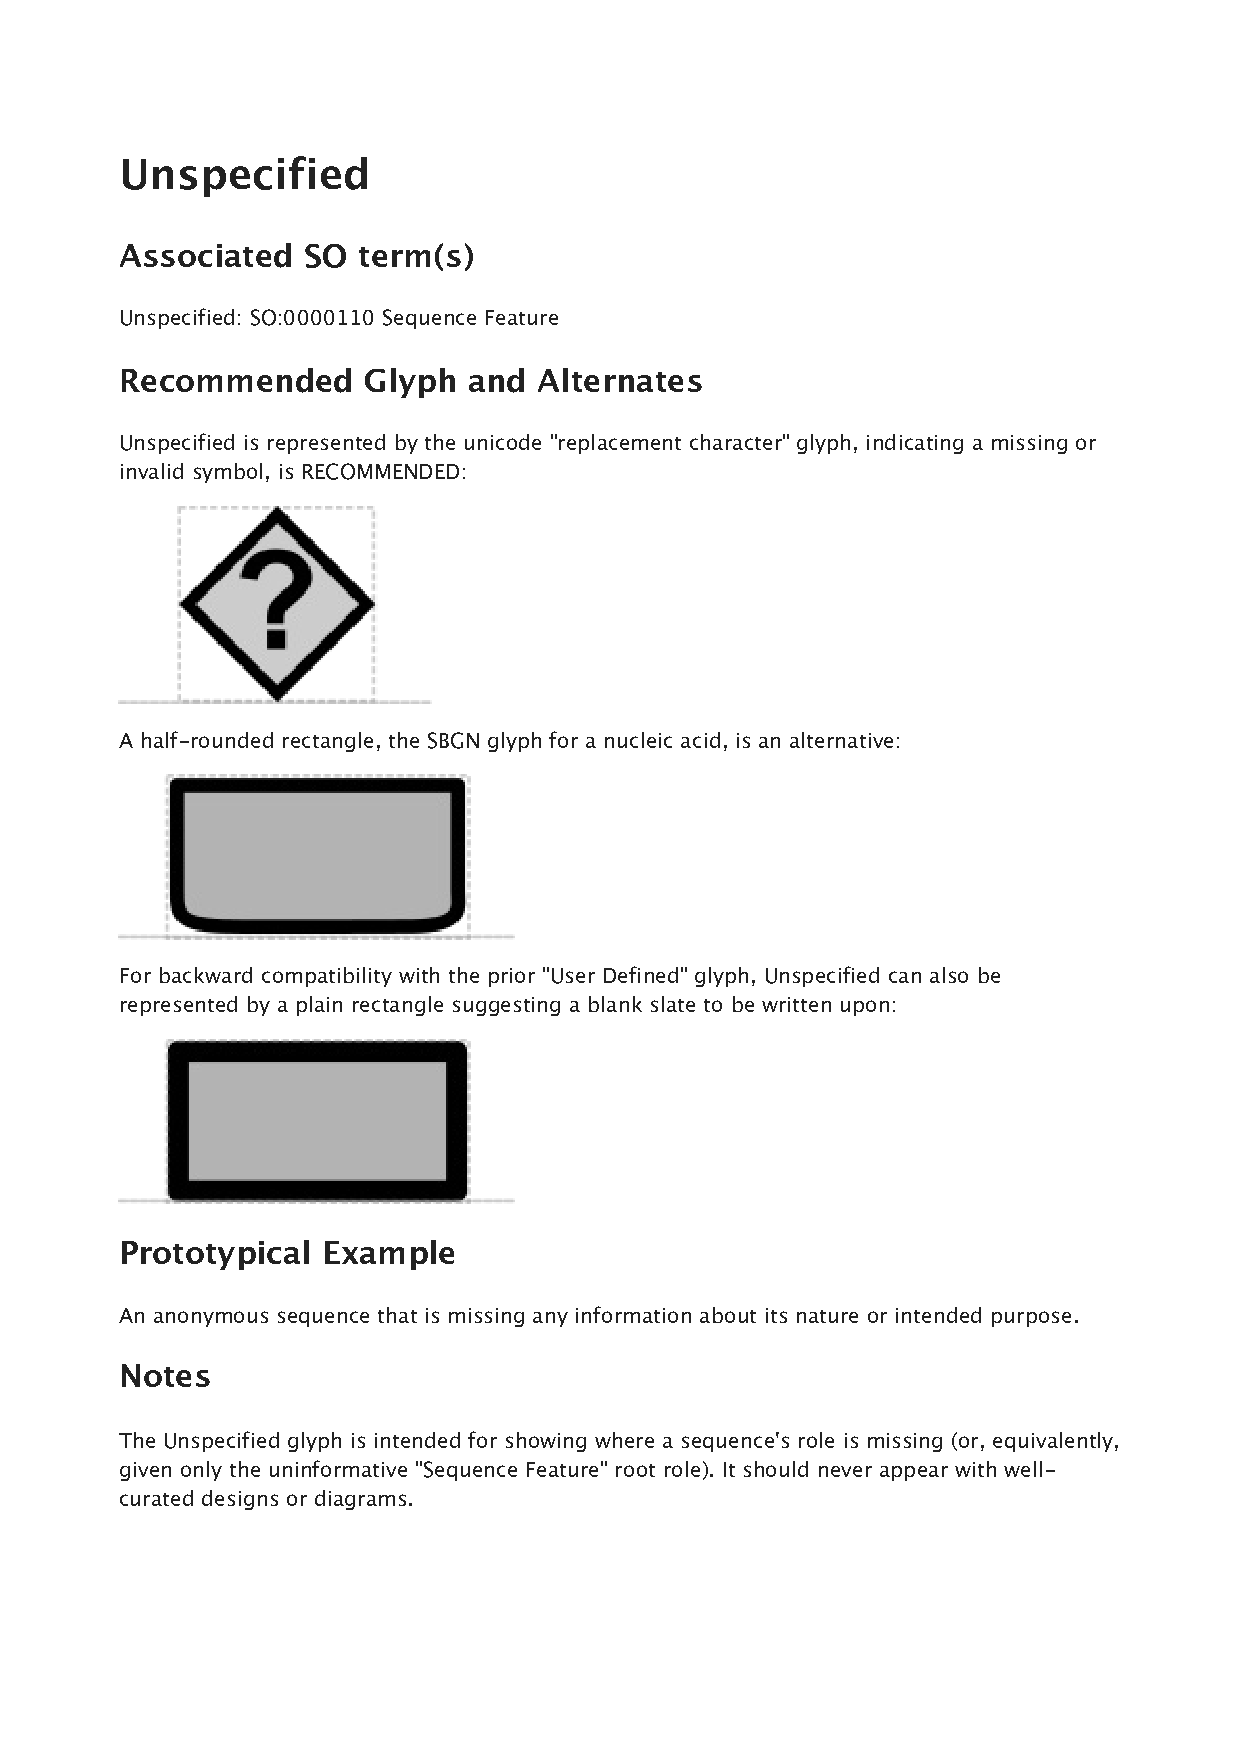
\includepdf[pagecommand={}]{glyphscript/Glyphs/unspecified.pdf}



\subsection{Molecular Species Glyphs}\label{apdx:sym:species}

These glyphs represent molecular species in a diagram, and include a bounding box (grey dashed box) but are not connected to any nucleic acid backbone.

% Autogenerated glyph page collection, do not edit by hand
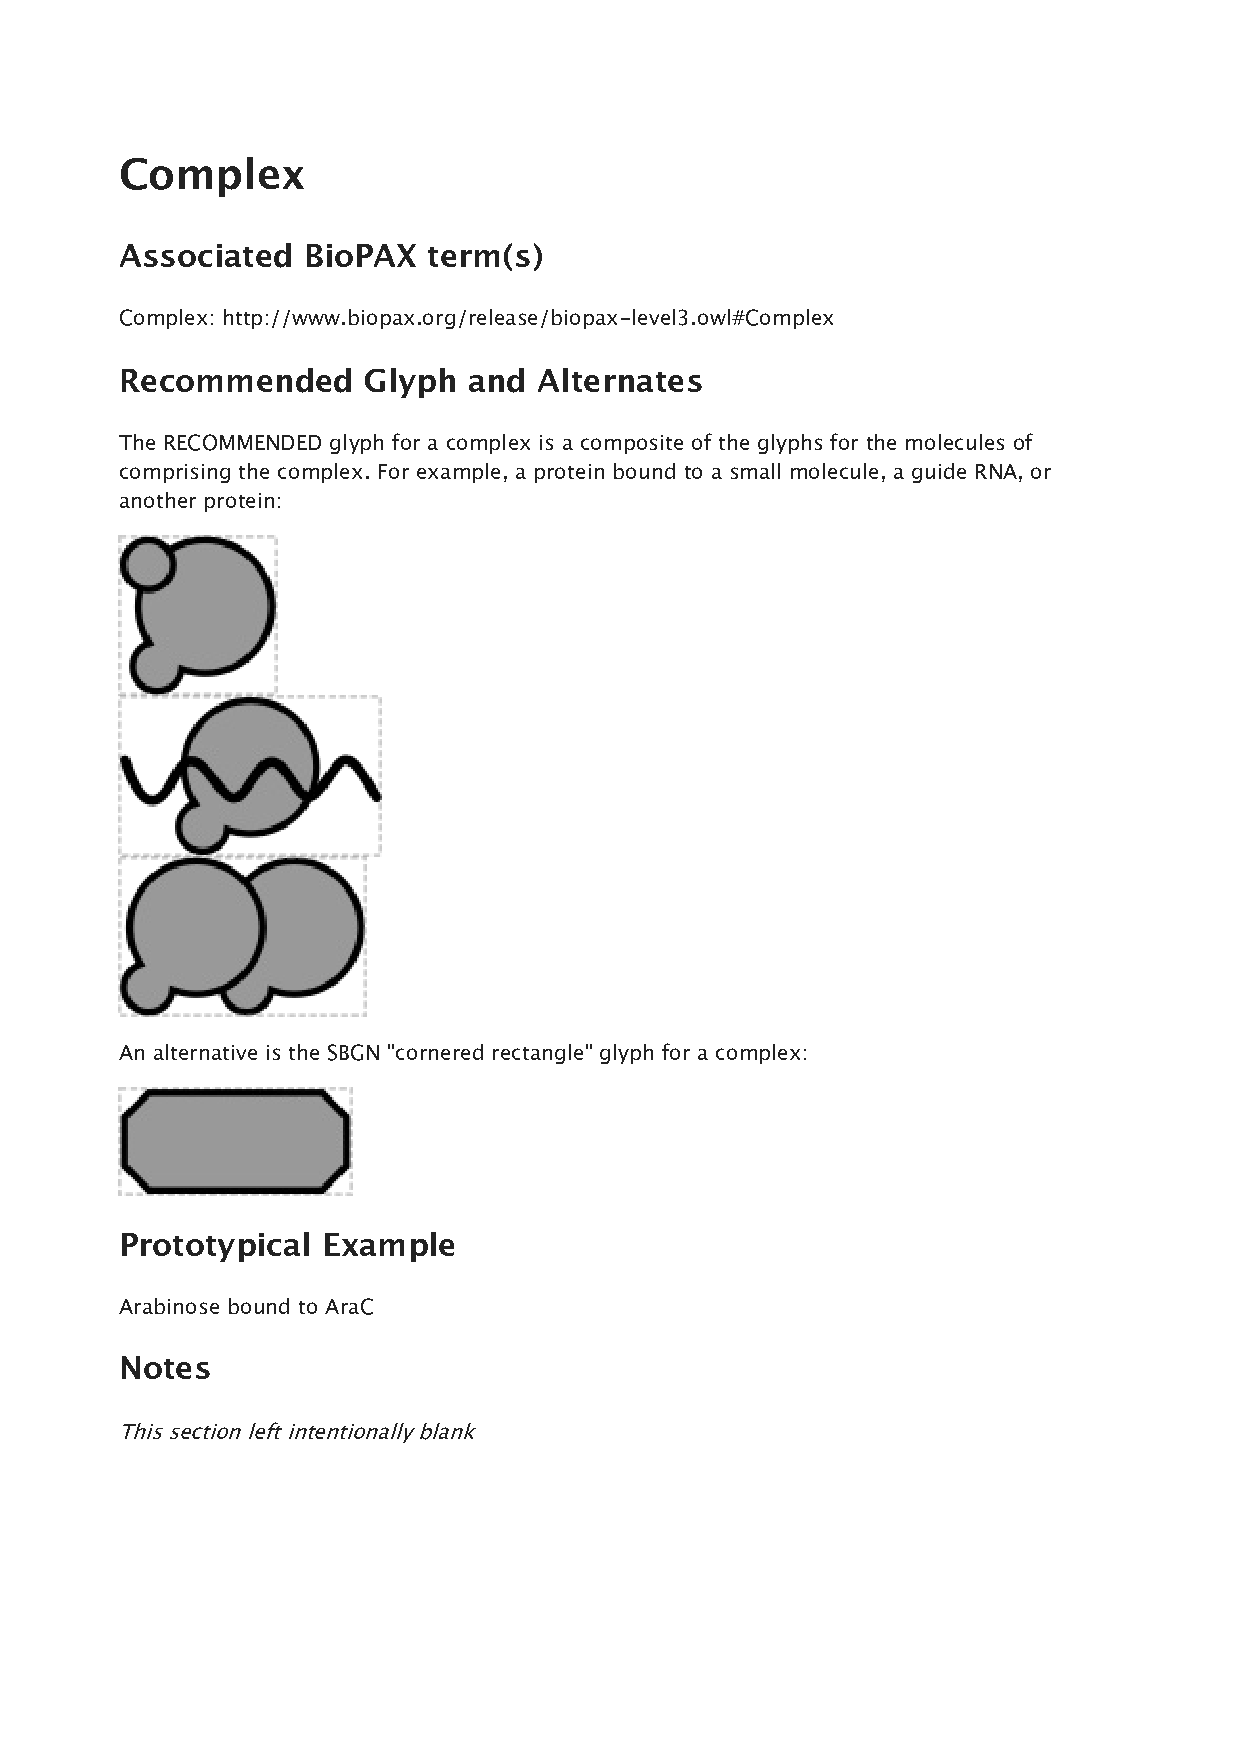
\includepdf[pagecommand={},pages={1-}]{glyphscript/Glyphs/FunctionalComponents/complex.pdf}
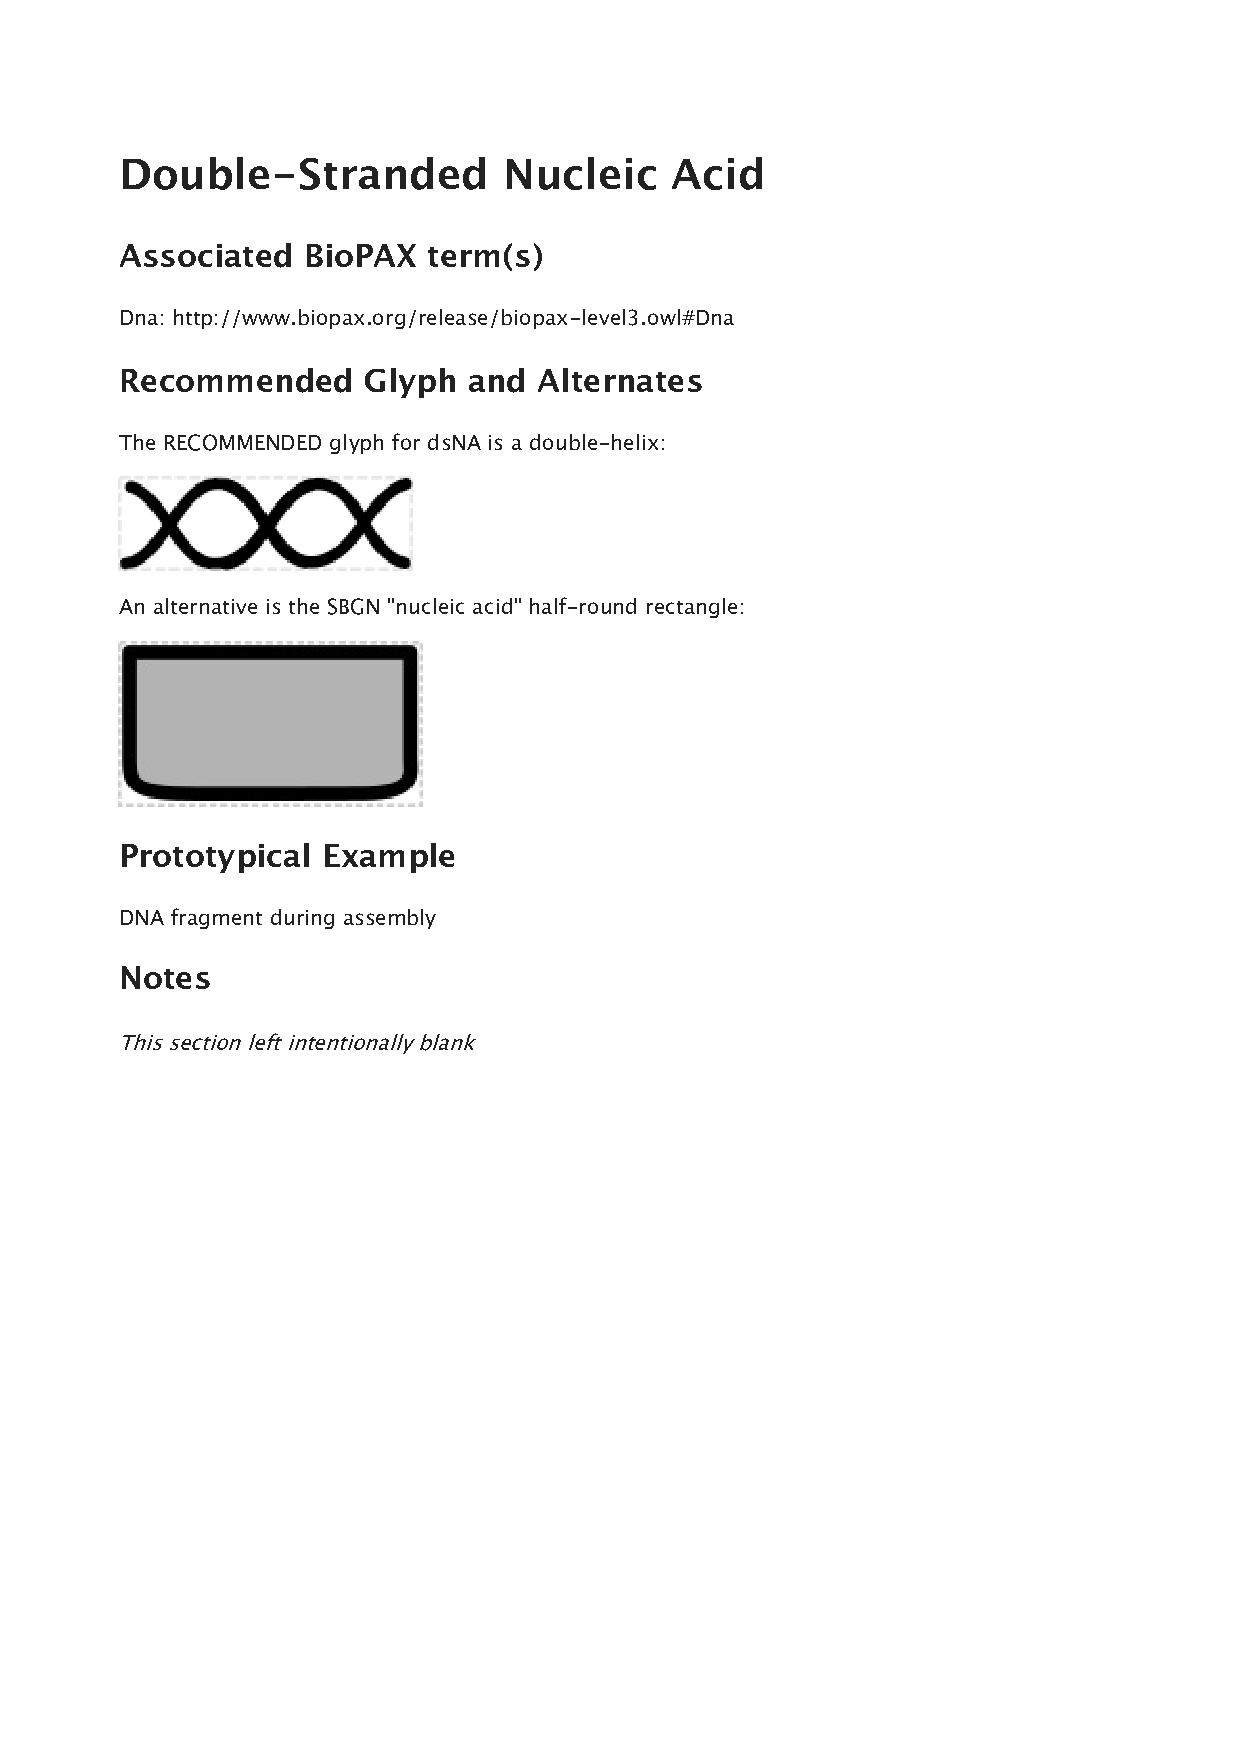
\includepdf[pagecommand={},pages={1-}]{glyphscript/Glyphs/FunctionalComponents/dsNA.pdf}
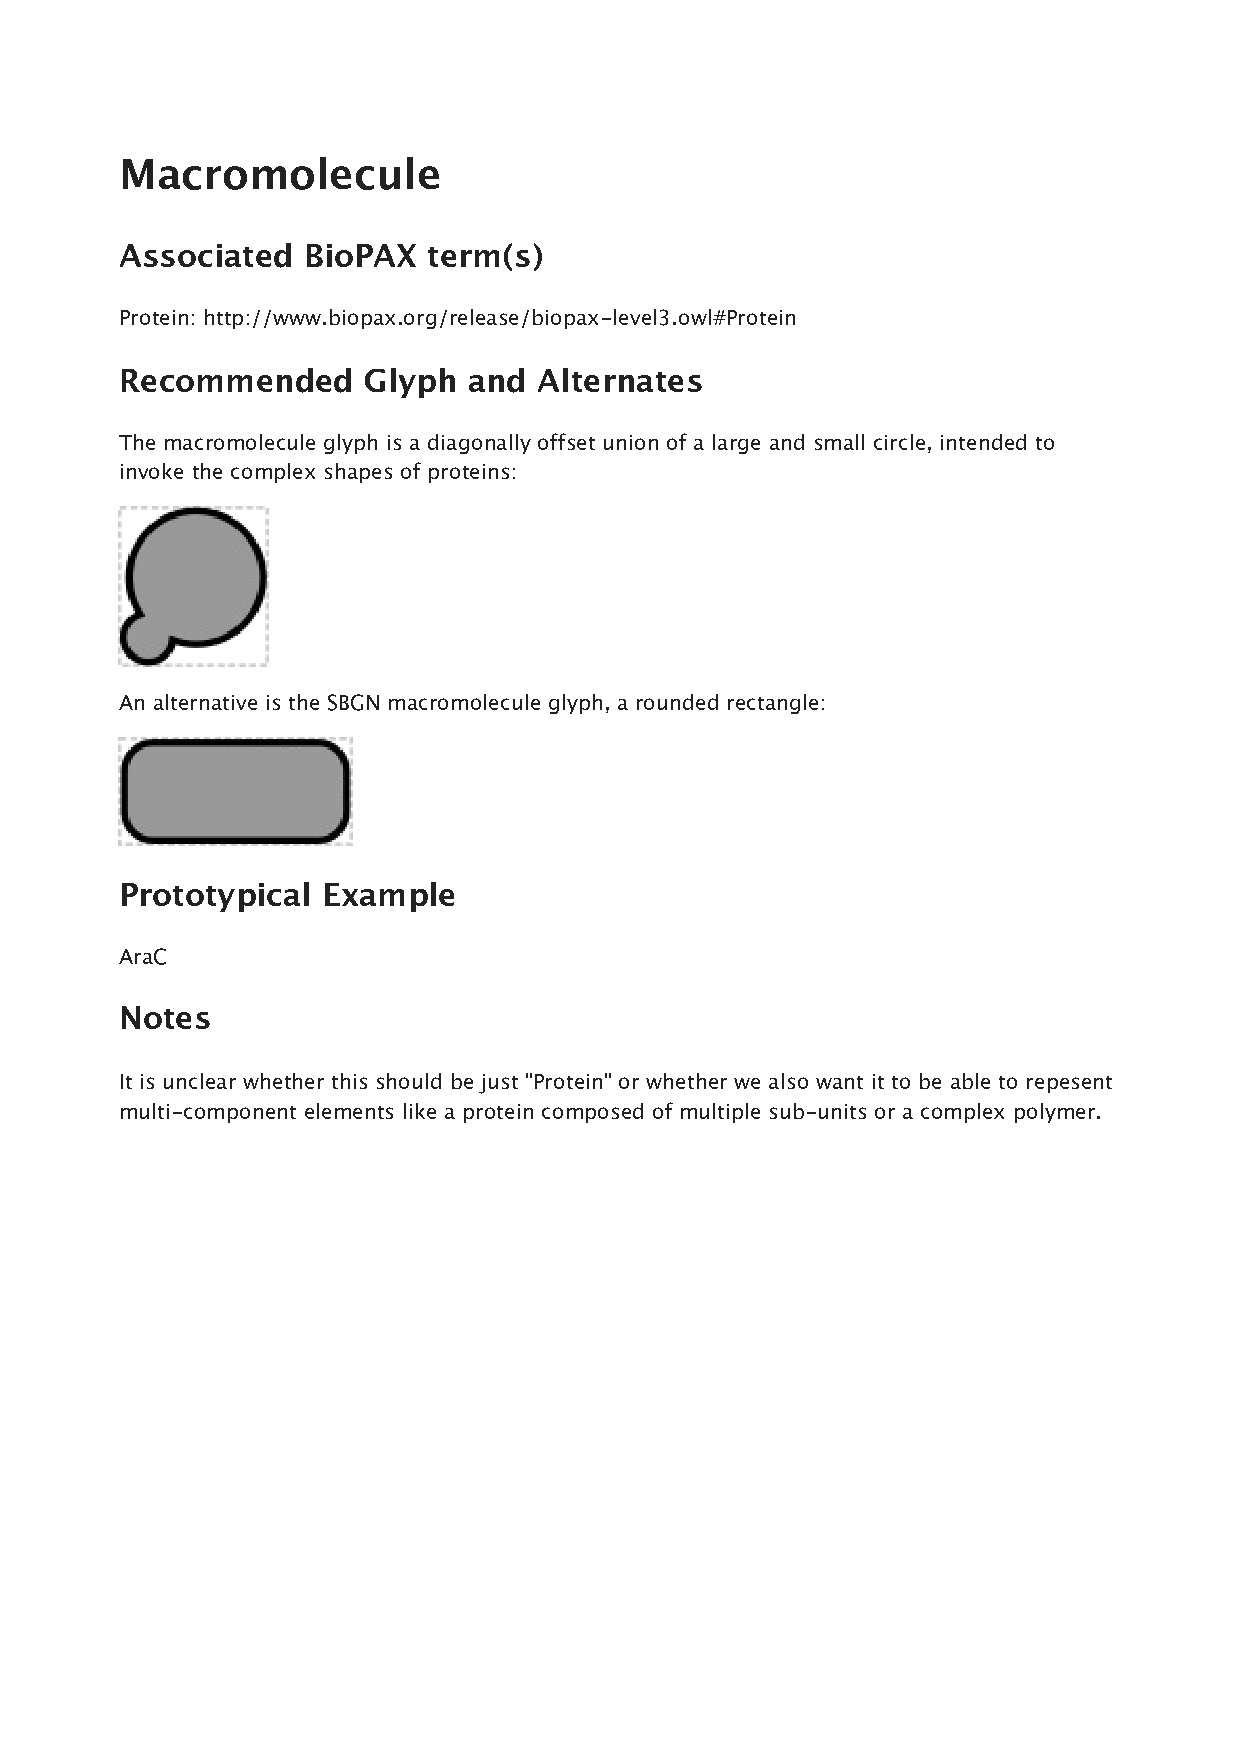
\includepdf[pagecommand={},pages={1-}]{glyphscript/Glyphs/FunctionalComponents/macromolecule.pdf}
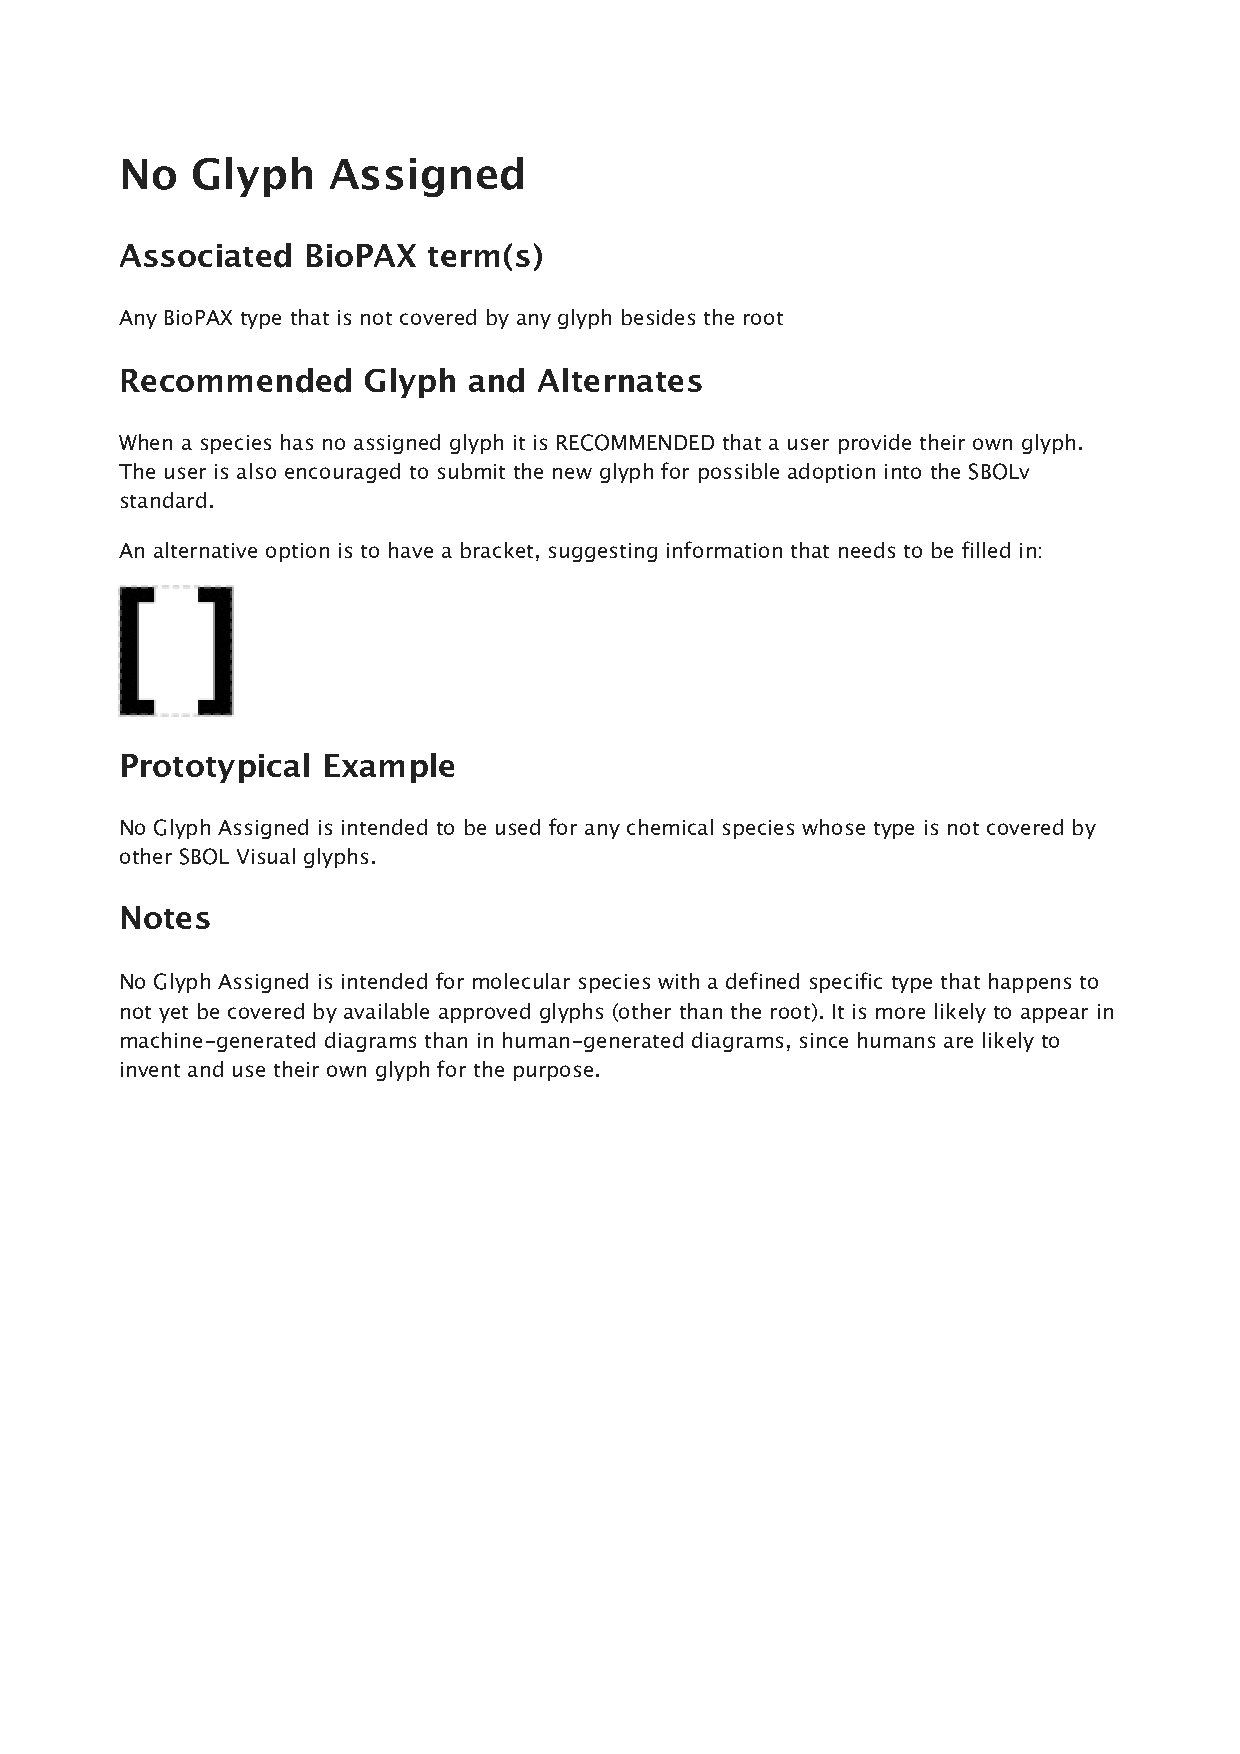
\includepdf[pagecommand={},pages={1-}]{glyphscript/Glyphs/FunctionalComponents/no-glyph-assigned.pdf}
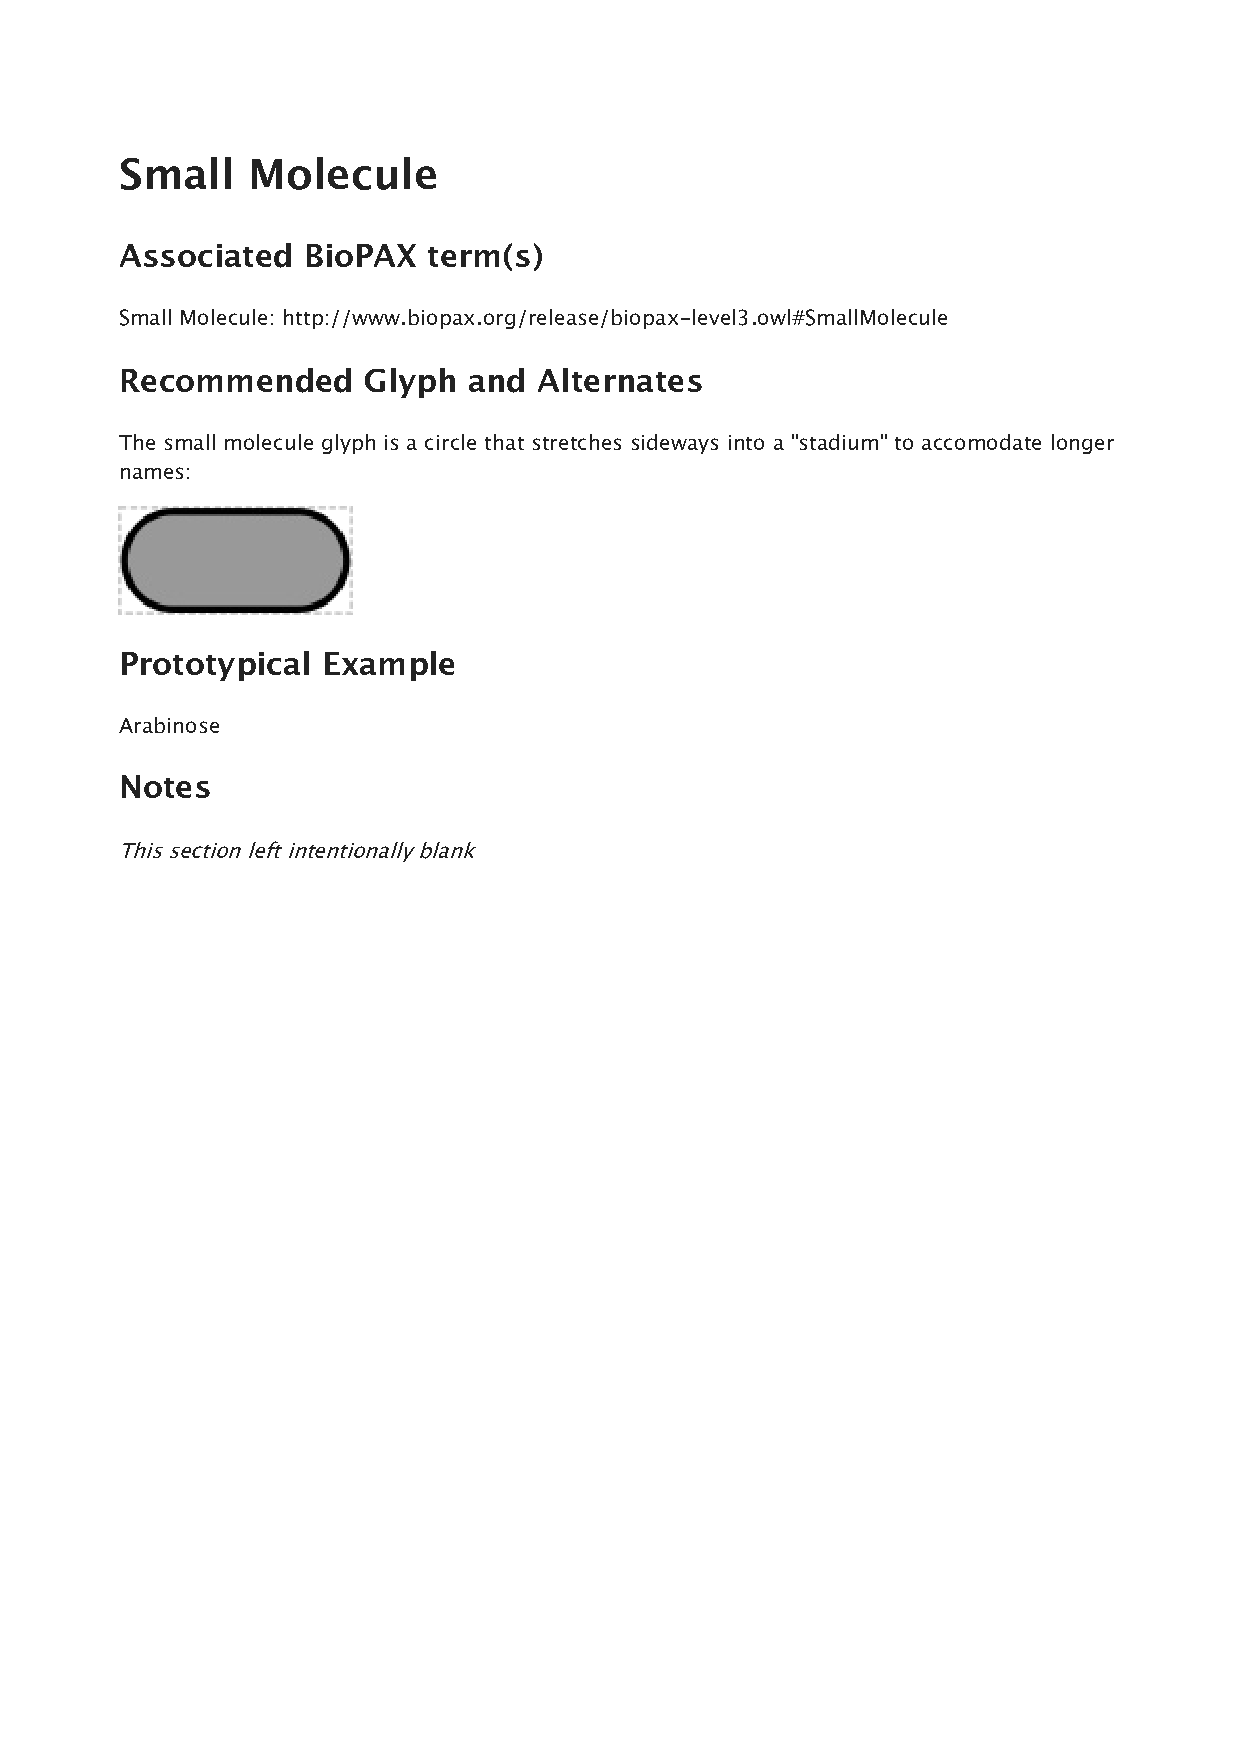
\includepdf[pagecommand={},pages={1-}]{glyphscript/Glyphs/FunctionalComponents/small-molecule.pdf}
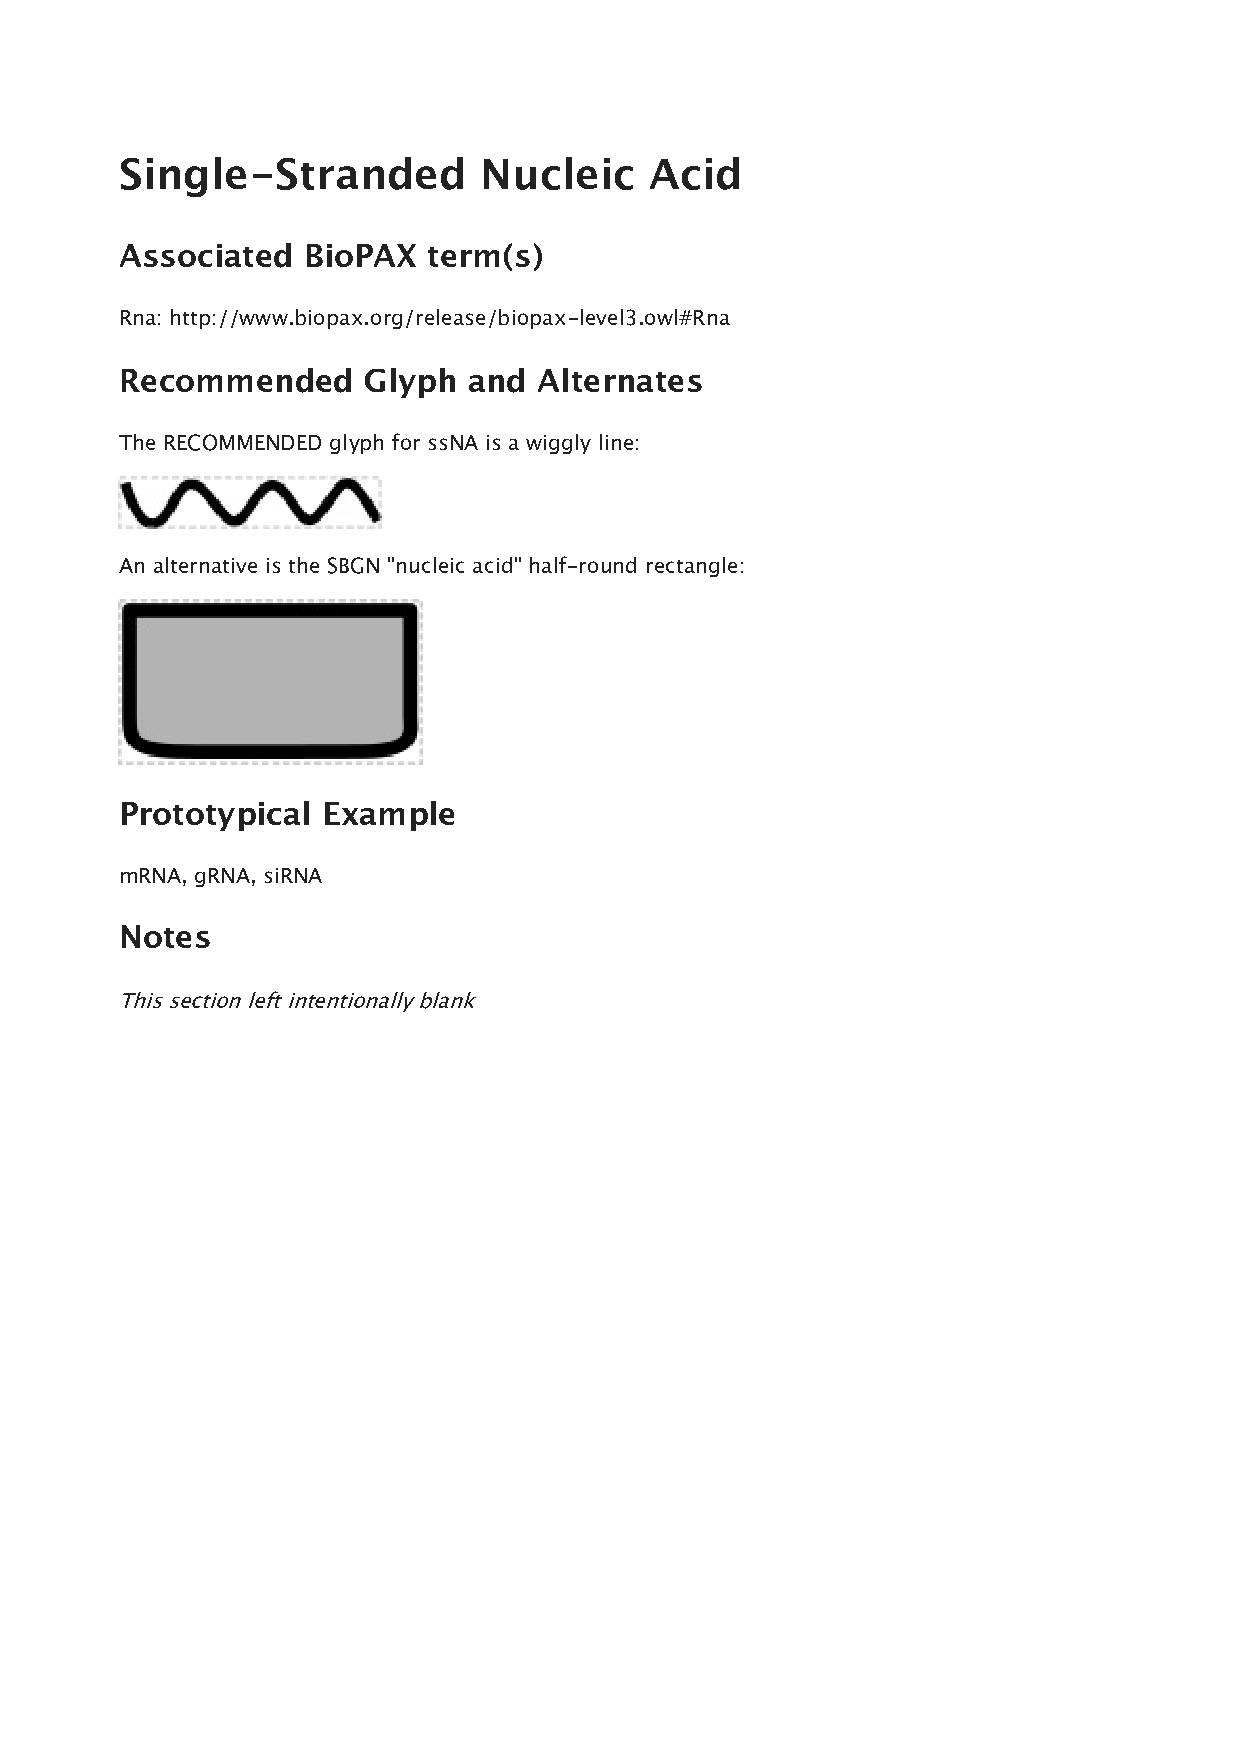
\includepdf[pagecommand={},pages={1-}]{glyphscript/Glyphs/FunctionalComponents/ssNA.pdf}
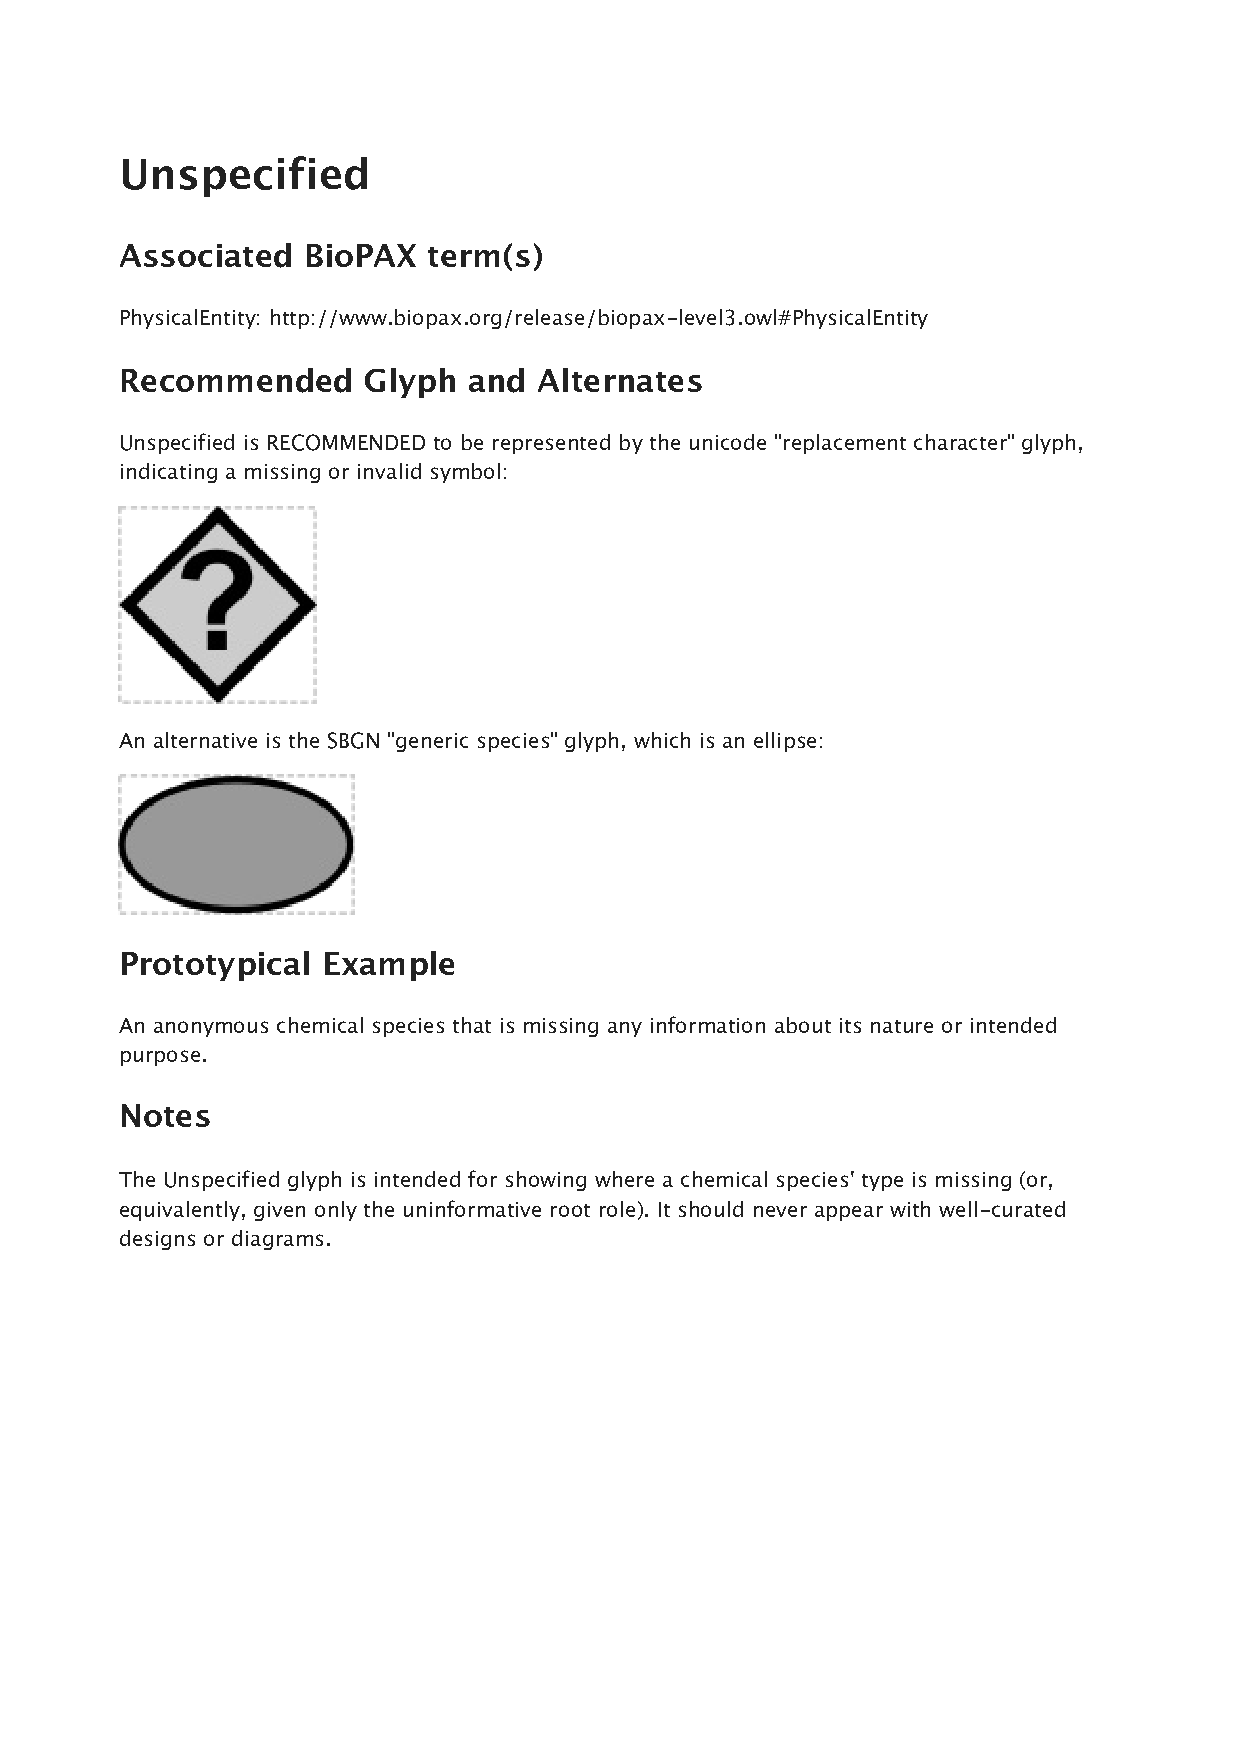
\includepdf[pagecommand={},pages={1-}]{glyphscript/Glyphs/FunctionalComponents/unspecified.pdf}



\subsection{Interaction Glyphs}\label{apdx:sym:interaction}

These glyphs are different forms of ``arrow'' representing interactions between sequence features and/or molecular species. As arrows, they are extensible and do not have a separately identified bounding box.

% Autogenerated glyph page collection, do not edit by hand
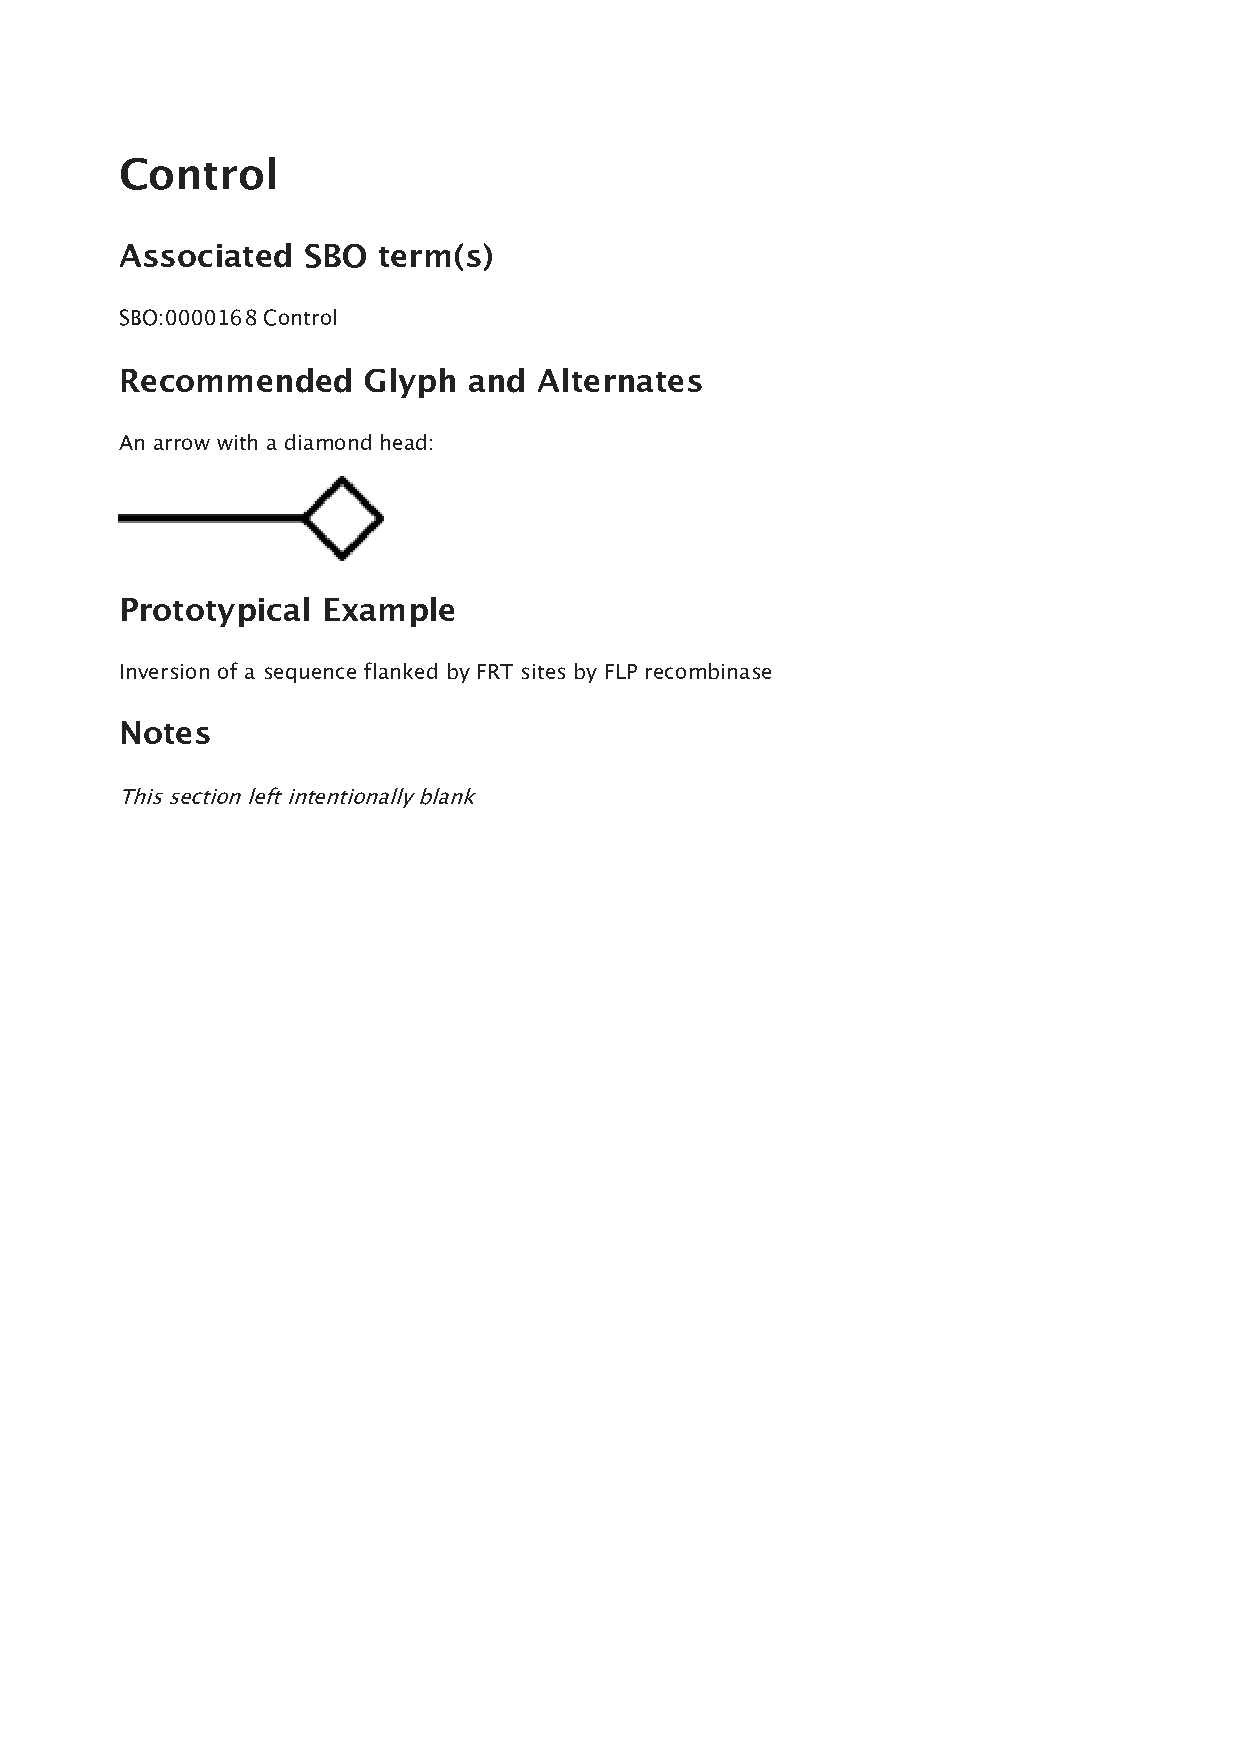
\includepdf[pagecommand={},pages={1-}]{glyphscript/Glyphs/Interactions/control.pdf}
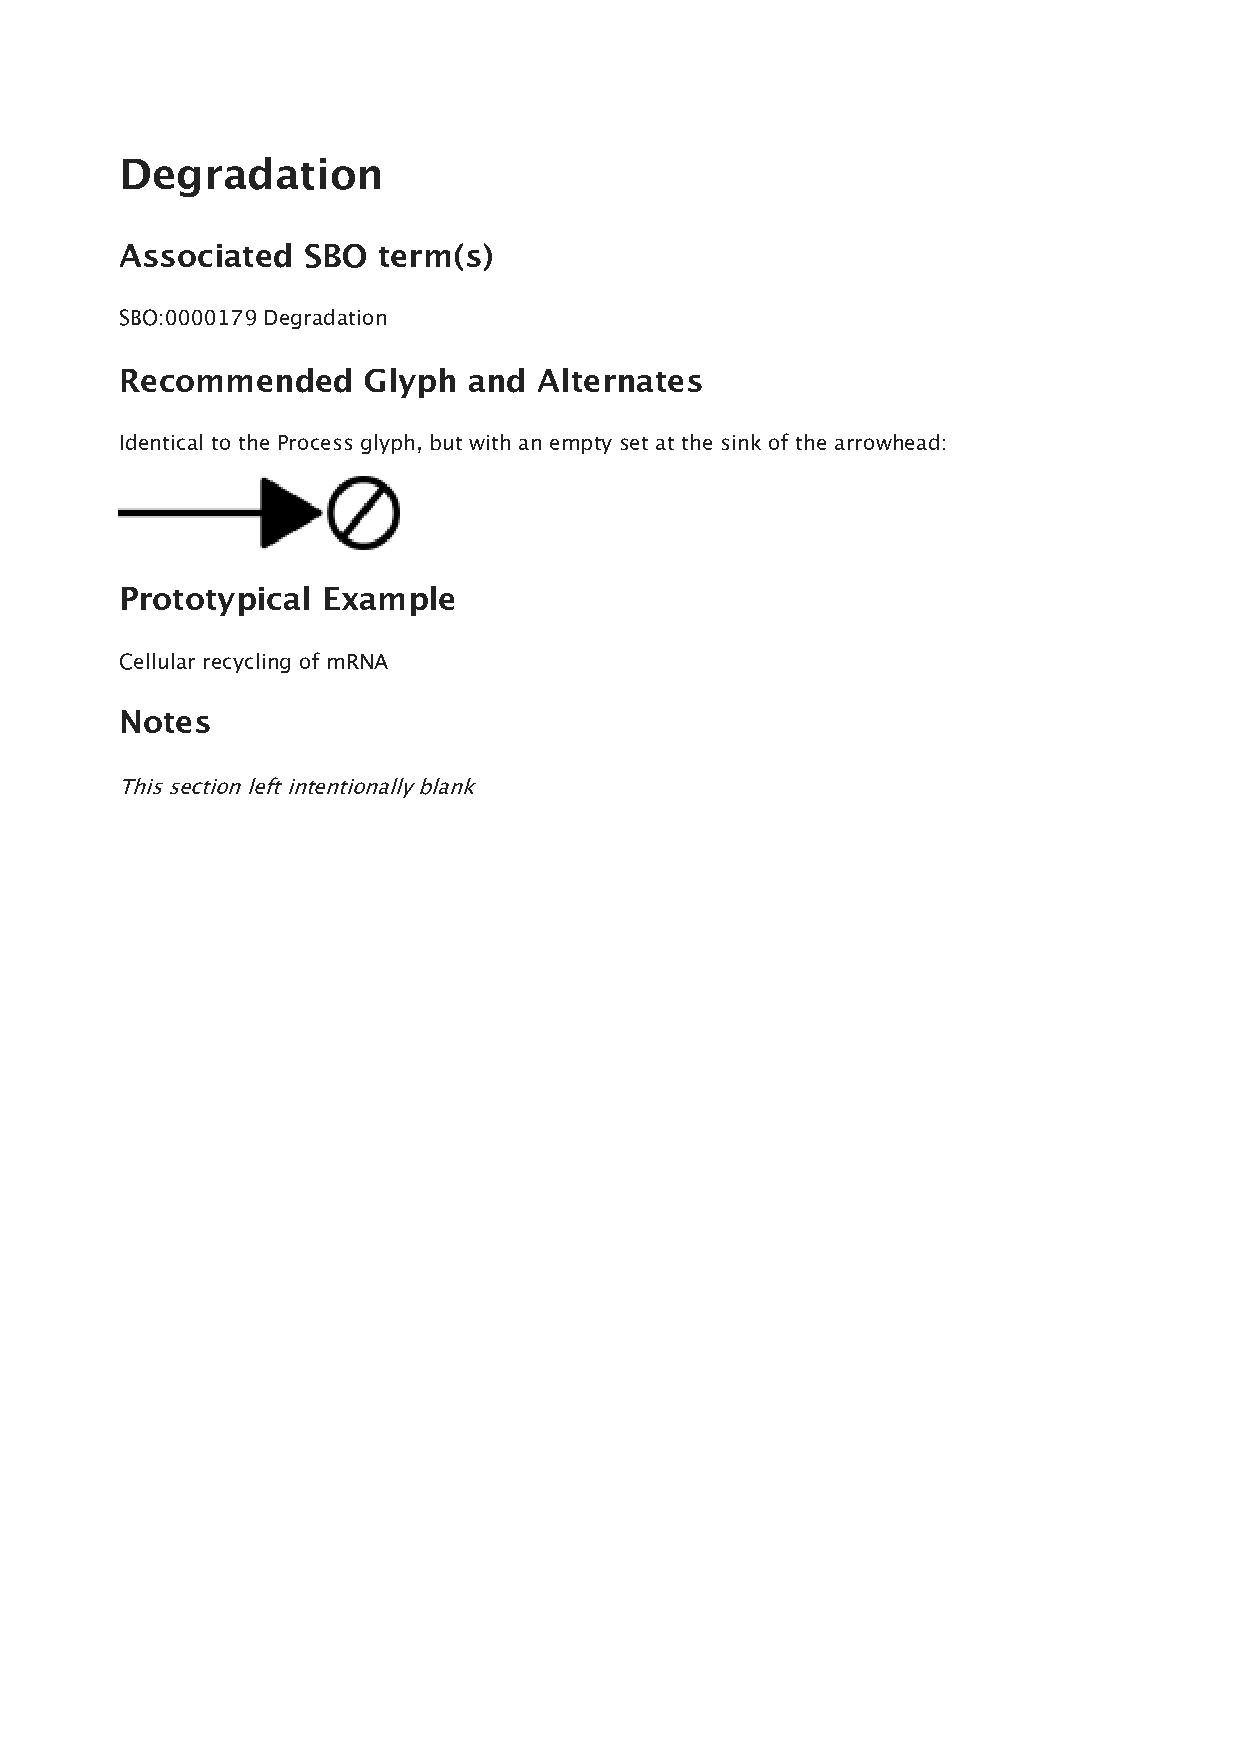
\includepdf[pagecommand={},pages={1-}]{glyphscript/Glyphs/Interactions/degradation.pdf}
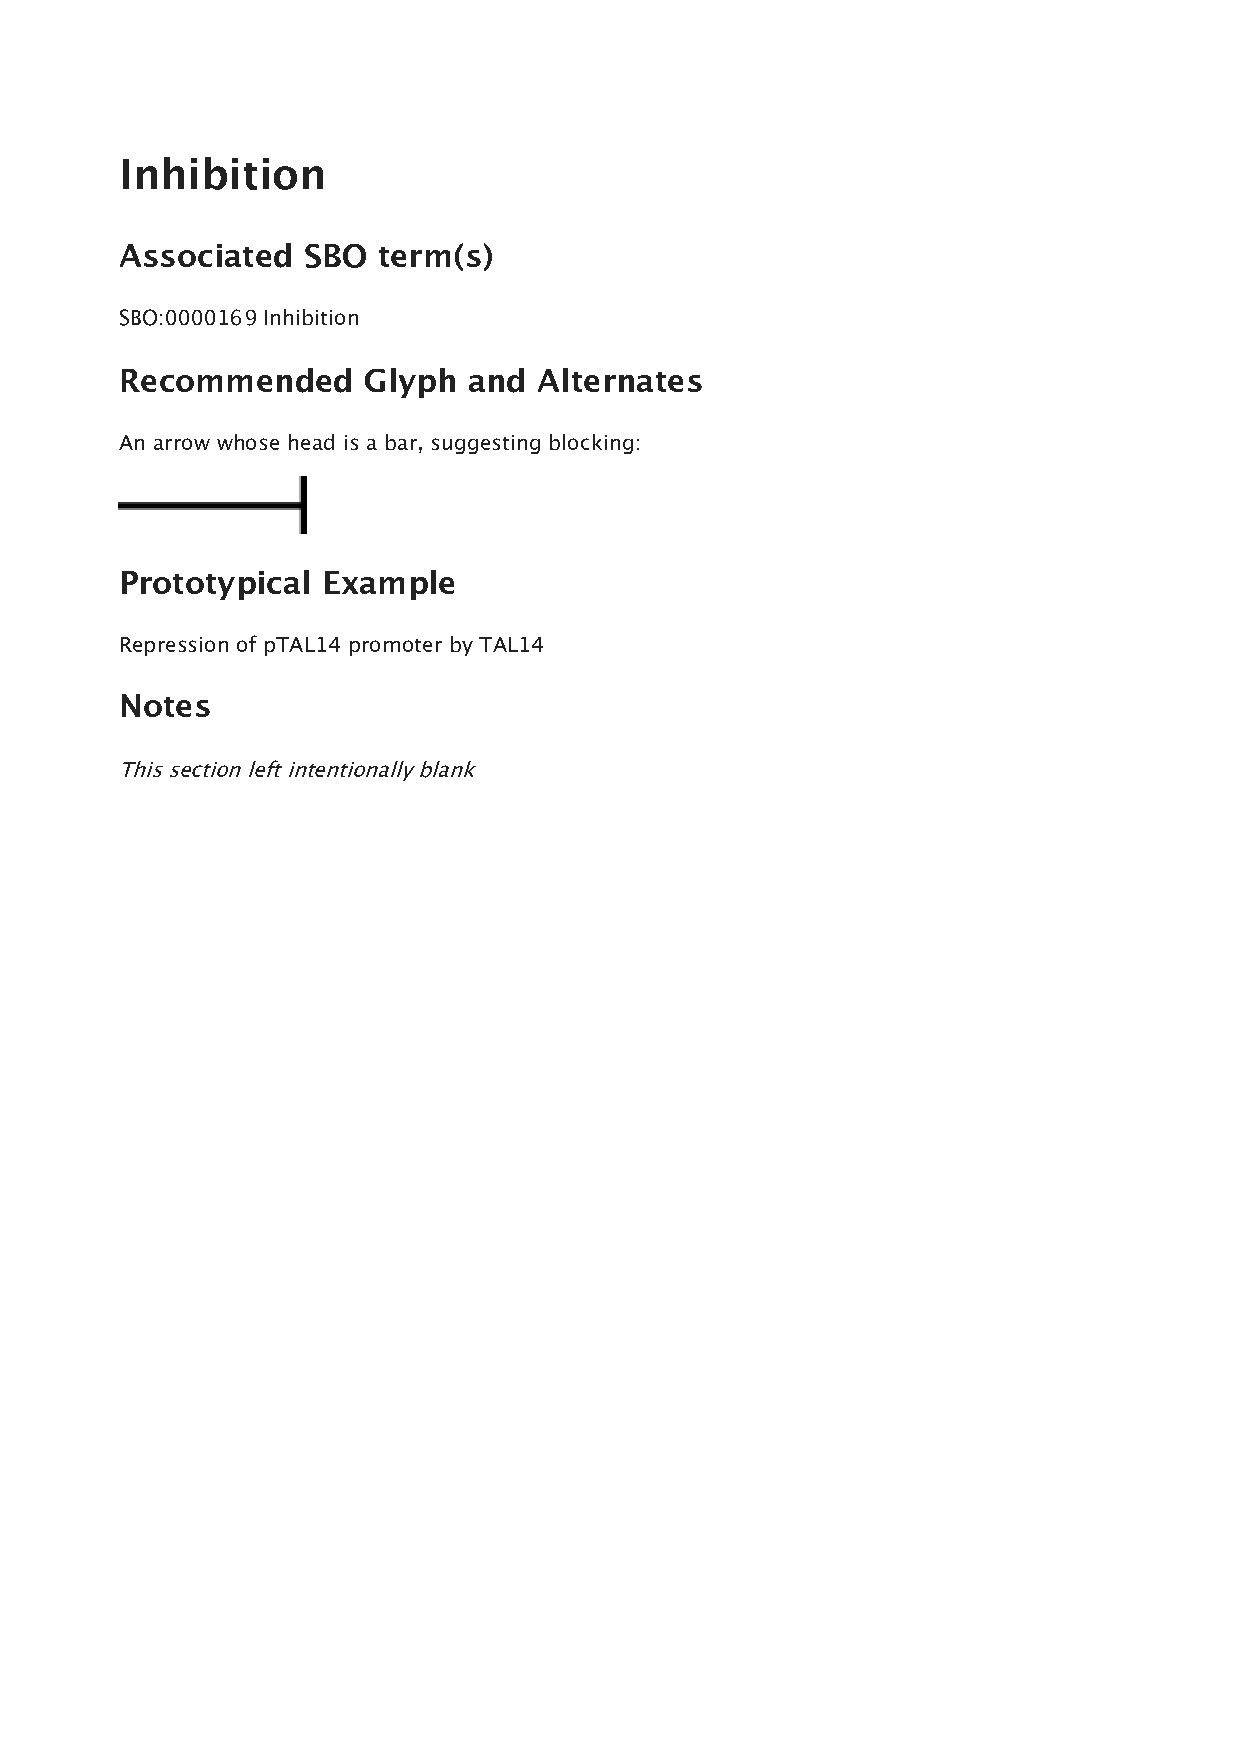
\includepdf[pagecommand={},pages={1-}]{glyphscript/Glyphs/Interactions/inhibition.pdf}
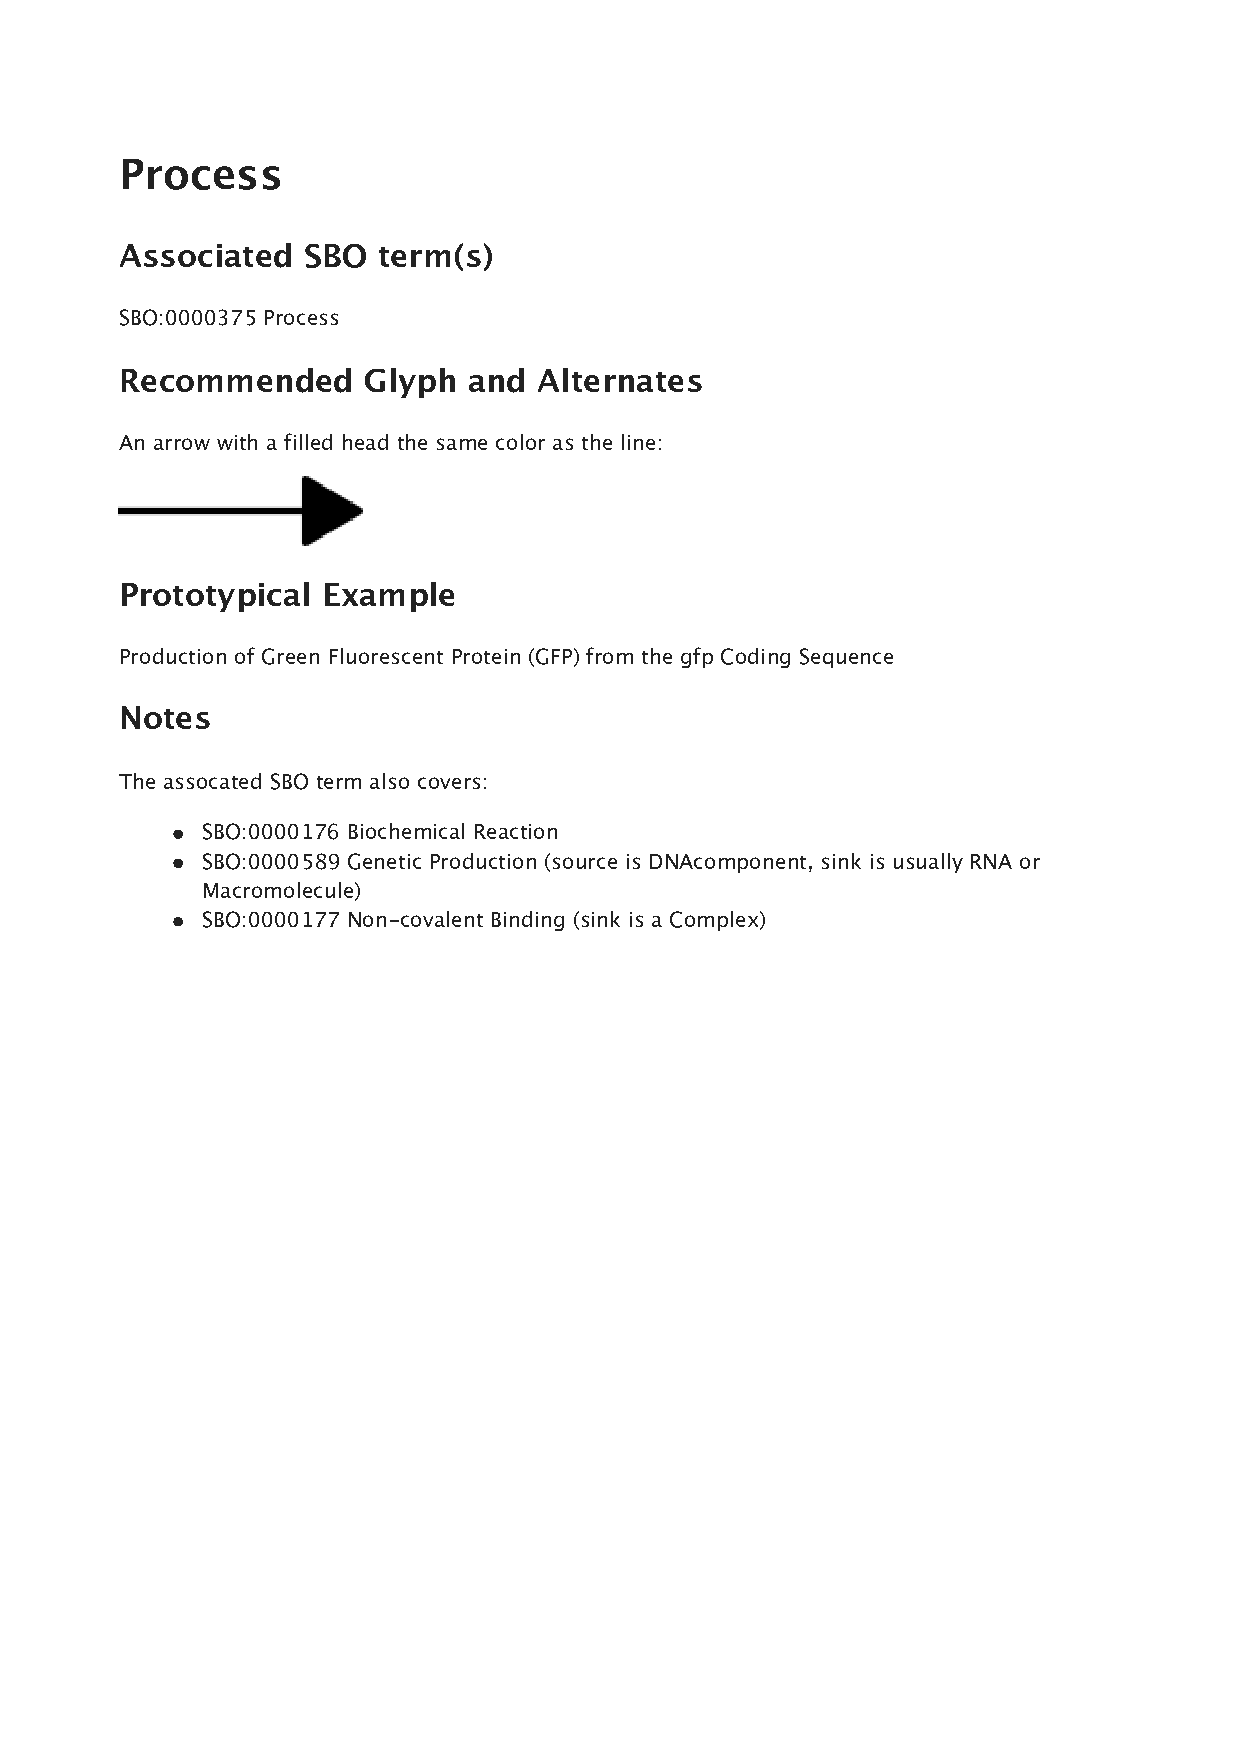
\includepdf[pagecommand={},pages={1-}]{glyphscript/Glyphs/Interactions/process.pdf}
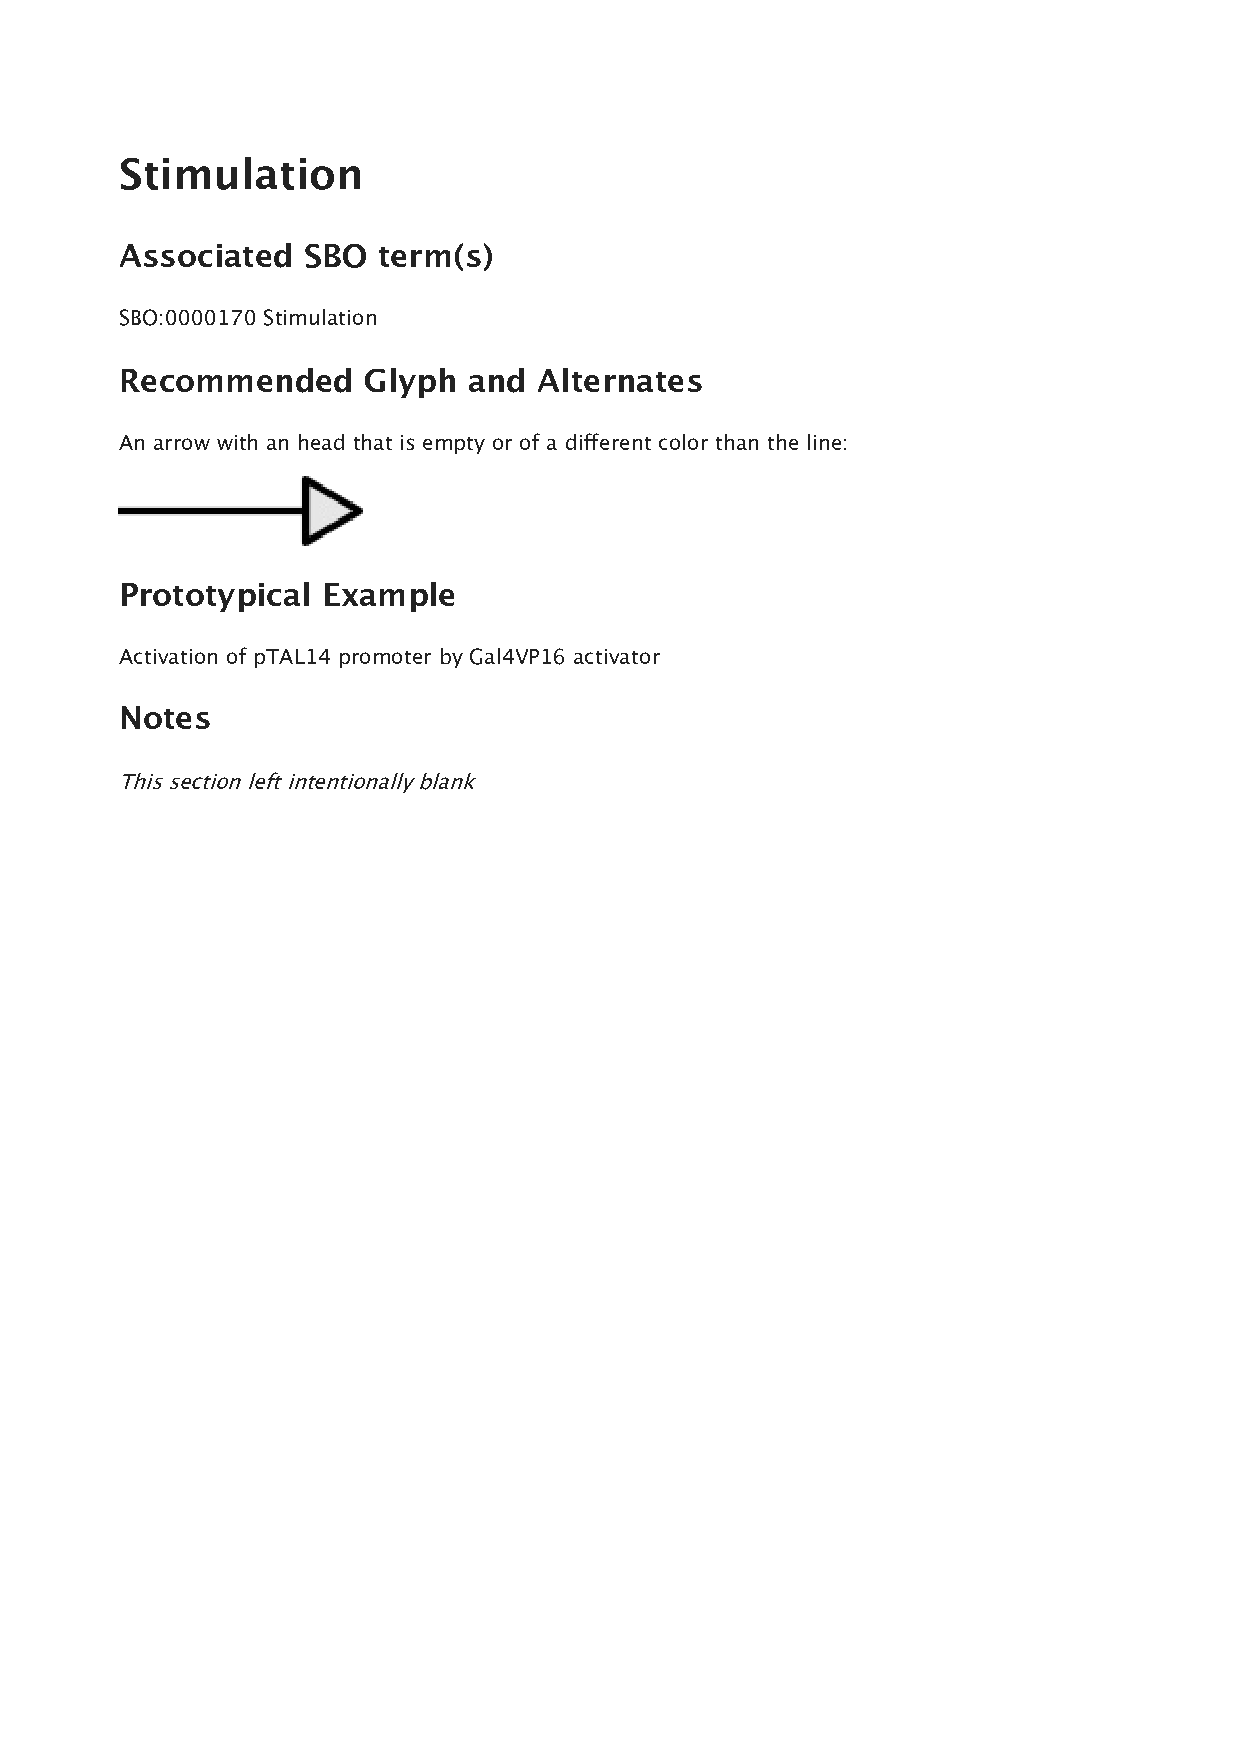
\includepdf[pagecommand={},pages={1-}]{glyphscript/Glyphs/Interactions/stimulation.pdf}

